\chapter{基于机器学习对南加州地区的地震中期预报}\label{chap:ml_seismic}

本研究围绕着利用机器学习探索时间序列数据展开,第\ref{chap:ml_sunspot}章基于一种特征(太阳黑子强度),第\ref{chap:ml_spring}章基于两种特征(泉流量和降雨量)。本章继续增加特征种类,利用机器学习对南加州地区的地震进行中期预报。

\section{研究背景}\label{sec:seism_introduction}

过去的几十年里,地球上发生了很多起大震。例如,2008年川滇地区7.9级地震,2011年日本东北9.0级地震,2015年尼泊尔7.8级地震,2017年墨西哥南部海岸8.2级地震,美国南加州7.1级地震等。倘若大震发生在人群居住密集区,可能会导致严重的人员伤亡和大量的财产损失。若能提前预报大震事件,就能够有效地拯救生命和减少财产损失。

地震预报一般涉及到几个要素,包括发生时间、经纬度、震级和发生的概率\citep{allen1976responsibilities}。地震预报是一个极具挑战性任务\citep{geller1997earthquakes}。一个多世纪以来地震学家仍然无法精准预报地震,很大一部分归咎于地震的自组织临界性。根据预报的时间长度,地震预报分为长期、中期和短期预报\citep{Pulinets2018What}。长期来看,强震的孕育需要需要上百年甚至上千年,现有的地震记录只有几十年,因此强震数值预报并不可靠。短期来看,地震预报非常容易受到的各种因素的干扰。因此,本章将重点放在中期地震数值预报。

地震数值预报离不开数据的支撑。数据来自地震目录、地震前兆(比如土壤中氡含量)、三分量地震仪测得的地震波、卫星数据等\citep{al2020application}。本章利用地震目录衍生出能够反映地震特征的地震因子。随着先进技术的发展,地震目录实现了实时更新,先进的方法和计算能力的提升为地震数值预报提供了新的机遇。

目前,预报地震已发展了很多方法,这些方法可分为由物理驱动的模型和由数据驱动的模型。由物理驱动的模型包括加速动量释放\citep{Ben2002Accelerated}、RTL(Region-Time-Length)算法\citep{Sobolev2007On}、ETAS(Epidemic-Type Aftershock Sequence)\citep{Ogata1986Statistical}等。由物理驱动的模型会因经验的局限性,难以拟合较为复杂的非线性特征,阻碍了对地震发生机制的进一步了解。

由数据驱动的方法因其强大的提取数据信息的能力,被越来越多地被应用到地震学中\citep{Alves2006Earthquake,Panakkat2007Neural,Madahizadeh2009prediction,Sunkara2009Model}。\citet{al2020application}系统性地总结了84篇科学论文,这些论文基于不同的数据和机器学习方法预报地震。\citet{al2020application}指出,被应用在地震学中的机器学习方法可被分为基于规则的方法、浅层机器学习和深层机器学习。基于规则的方法包括模糊逻辑\citep{zhong2010prediction,zamani2013application,mirrashid2014earthquake}和模糊神经网络\citep{Lopez2019Evolutionary}。浅层机器学习包括SVR\citep{asencio2017temporal}、RF\citep{asim2017earthquake}、DT\citep{asencio2017temporal}、KNN\citep{Panakkat2007Neural,asencio2017temporal}、BPNN\citep{Panakkat2007Neural,Narayanakumar2016A}、径向基神经网络\citep{Alexandridis2014Large}、概率神经网络\citep{Adeli2009A}、聚类\citep{shodiq2018neural}等。深层神经网络包括RNN\citep{Panakkat2009Recurrent,asim2017earthquake}、LSTM-RNN\citep{Wang2017Earthquake,Bhatia2018EARTHQUAKE,berhich2020lstm}、多层的神经网络\citep{huang2018large}等。

地震因子是指与地震发生有关的地球物理信息的特征。已有一些研究提出使用地震因子进行地震预测\citep{Panakkat2007Neural,martinez2013determining,reyes2013neural,morales2013earthquake,asencio2016sensitivity}。例如,\citet{reyes2013neural}提出了基于一些地震因子作为地震预测的输入;\citet{martinez2013determining}结合了\citet{Panakkat2007Neural}中的地震因子,使用特征选择方法分析了地震因子与二元分类(地震发生与否以及是否发生大震)的相关性;\citet{asencio2016sensitivity}基于几种不同的监督学习模型,同时利用计算的$b$值调整地震因子,进而提高地震预测的精度;\citet{asim2018seismic}利用集成模型基于地震因子预报未来15天内是否会出现5.0级以上的地震。

这项工作的重点是利用几个有监督的机器学习模型,基于各种地震因子作为模型的输入,以提高地震预测的准确性,这些研究关注的是中小震。为了实现预报大震任务,本研究采取了LSTM-RNN\citep{Wang2017Earthquake,Bhatia2018EARTHQUAKE,berhich2020lstm}和其他几种机器学习算法(SVR、LR、RF、DT、KNN、GBRT、ETR)对地震进行中期预报。本章选择美国南加州地区作为研究区域。该地区属于地震孕育区(地震孕育区是基于地震震源和浅层地质构造背景的空间分布)。南加州地震目录记录的时间长达$\sim$90年,是一个较为理想的地震研究区域。

本章结构安排如下。第\ref{sec:seism_data_method}节介绍了数据与方法,具体包括研究区域介绍、地震目录特征描述、地震因子的计算、时空窗口法、数据的预处理过程等。第\ref{sec:seism_result}节描述地震预报的试验过程,并将试验结果可视化。第\ref{sec:seism_conclusion}节对本章地震预报进行了小结。

\section{数据与方法}\label{sec:seism_data_method}

\subsection{研究区域}\label{sec:seism_area}

加利福尼亚州位于北美和太平洋板块之间,地壳运动频繁,是地震多发地带。南加州地区的地震目录记录时间较长(\sim 90年),且地震记录相对较为完备,故本研究选择南加州地区作为研究区域,地理范围在$[\SI{32\cirl}{N}-\SI{37}{N}]$和$[\SI{114}{W}-\SI{122}{W}]$。图\ref{fig:seism_california}绘制了南加州地区区域构造和地震目录中记录地震的震级和发生位置。

\begin{figure}[!htbp]
  \centering
  \includegraphics[width=0.70\textwidth]{Img/chap5_seism/seism_carlifornia.pdf}
  \bicaption[南加州地区区域构造]{南加州地区区域构造。}{Tectonics of the Southern California area.}
  \label{fig:seism_california}
\end{figure}

\subsection{地震目录}\label{sec:seism_catolog}

\begin{table}[!htbp]
  \bicaption[1932年至2021年期间研究区域内7级以上的地震]{1932年至2021年期间研究区域内7级以上的地震。}{Earthquake with magnitude no less than 7 in the study area from 1980 to 2021.}
  \label{tab:seism_magnitude_7}
  \centering
  \footnotesize
  \begin{tabular}{ccccc} 
    \toprule
    发生时间 & 纬度(N) & 经度(W) & 震级 \\
    \midrule
    1952-07-21 11:52:14 & 34.958 & 118.998 & 7.5 \\
    1992-06-28 11:57:34 & 34.200 & 116.437 & 7.3 \\
    1999-10-16 09:46:44 & 34.603 & 116.265 & 7.1 \\
    2010-04-04 22:40:42 & 32.286 & 115.295 & 7.2 \\
    2019-07-06 03:19:53 & 35.770 & 117.599 & 7.1 \\
    \bottomrule
  \end{tabular}
\end{table}


地震目录来自南加州地震数据中心(Southern California Earthquake Data Center,简称SCEDC)\footnote{数据来源:\href{https://service.scedc.caltech.edu/ftp/catalogs/}{https://service.scedc.caltech.edu/ftp/catalogs/}}。地震目录从1932年1月1日开始记录,2021年9月19日截至,位于研究区域内一共有831,906条数据。每条记录包含以下信息:
\begin{itemize}
  \item[1] 发生时间(年,月,日,时,分,秒);
  \item[2] 发生地点,分别为纬度(N)、经度(E)、深度(向下);
  \item[3] 震级。
\end{itemize}

在地震预报中,重点关注大震。表\ref{tab:seism_magnitude_7}列出研究区域内7级以上的地震。由表\ref{tab:seism_magnitude_7}可知,近三四十年来,每隔$\sim$10年该地区会发生7级以上的地震。

\begin{figure}[!htbp]
  \centering
  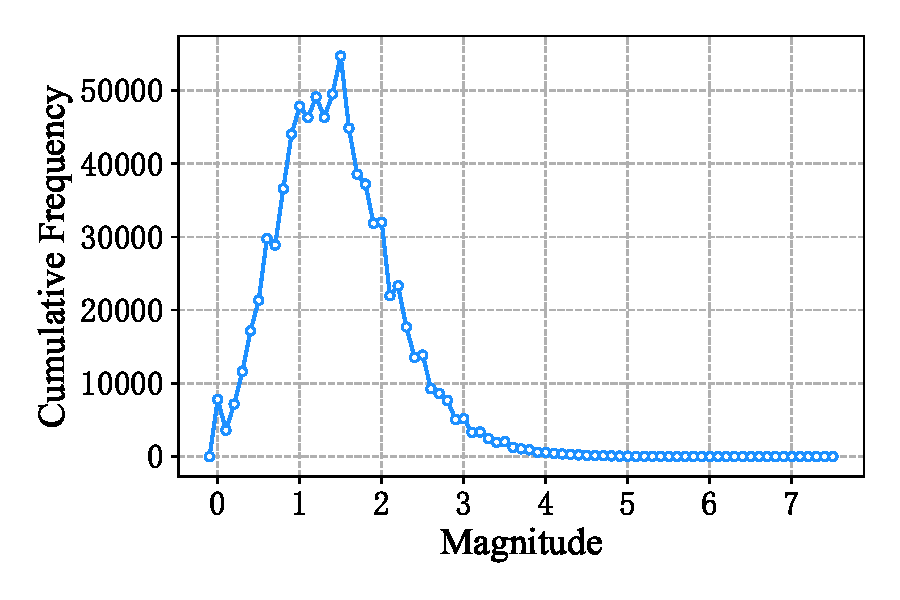
\includegraphics[width=0.60\textwidth]{Img/chap5_seism/seism_m_f.pdf}
  \vspace{-0.5cm}
  \bicaption[震级与频度的关系]{震级与频度的关系。}{Relationships between magnitude and cumulative frequency.}
  \label{fig:seism_m_f}
\end{figure}

在给定的研究区域内,频度和地震事件的震级服从Gutenberg-Richter法则\citep{Gutenberg1994Frequency,Panakkat2007Neural}。该法则的数学表达形式如下:
\begin{equation}\adddotsbeforeeqnnum
  \label{eq:seism_Gutenberg-Richter}
  \log N=a-bM.
\end{equation}
其中,$N>0$,$N$指震级不小于阈震级$M_c$的地震事件的累积数量。$b$值为斜率,由震级和频度决定。Gutenberg-Richter法则是指,随着震级逐渐增大,地震频度出现指数级下降\citep{Asim2018Earthquake}。图\ref{fig:seism_m_f}绘制了南加州地区震级与频度关系图,发现小震发生的次数远超出大震,但震级在小于2时,图\ref{fig:seism_m_f}并不满足Gutenberg-Richter法则,小震存在缺失的情况。

公式\ref{eq:seism_Gutenberg-Richter}可知,$b$值反映了震级频度关系,$b$值越小表示较大震级的地震发生频次越高。\citet{schorlemmer2005variations}研究发现,断层类型与$b$值存在显著的关系,因此$b$值能够体现研究区域的应力水平。$b$值一般可以通过两种方法获取,分别为最小二乘(Least Square,简称LS)法和最大似然估计( Maximum Likelihood Estimation,简称MLE)法。图\ref{fig:seism_b_m_1932_2021}绘制了1932年至2021年期间不同起算震级下利用MLE法得到的$b$值。图\ref{fig:seism_logn_m_1932_2021}则绘制了Gutenberg-Richter法则的关系图。图\ref{fig:seism_b_m_1932_2021}和图\ref{fig:seism_logn_m_1932_2021}拐角处的震级可看作是阈震级。综合两图的效果,发现从1932年至2021年期间,南加州地震目录中3级以上的地震基本完备,原始地震目录减少到24,865条。

\begin{figure}[!htbp]
  \centering
  \begin{subfigure}[b]{0.4\textwidth}
    \caption{$b$值与起算震级的关系} 
    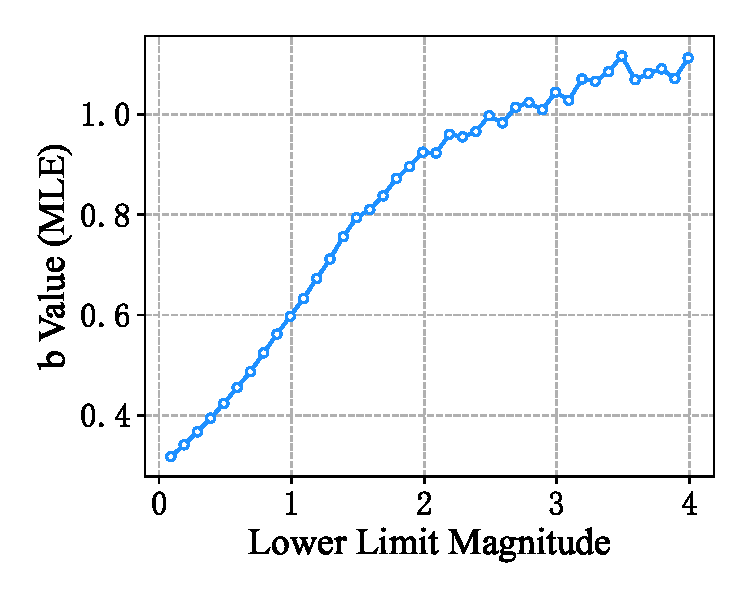
\includegraphics[width=\textwidth]{Img/chap5_seism/seism_b_1932_2021.pdf}
    \label{fig:seism_b_m_1932_2021}
  \end{subfigure}   
  ~
  \begin{subfigure}[b]{0.4\textwidth}
      \caption{$\log N=a-bM$}
      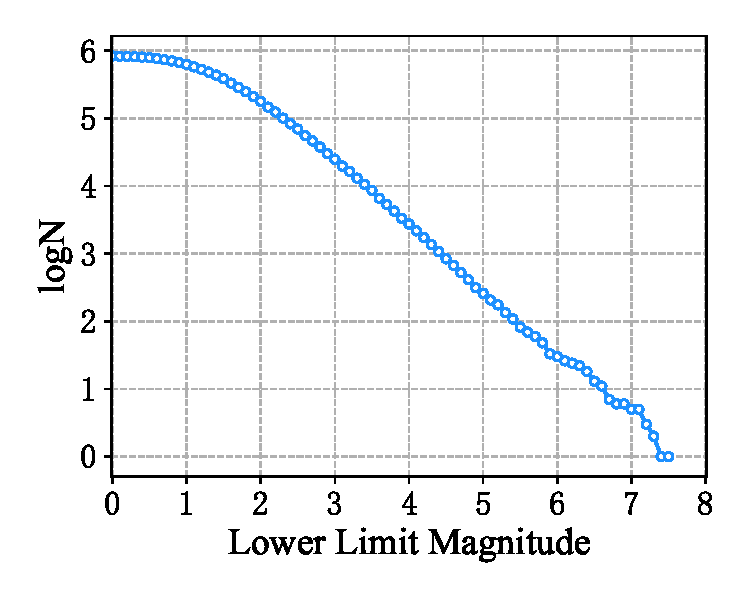
\includegraphics[width=\textwidth]{Img/chap5_seism/seism_logN_1932_2021.pdf}
      \label{fig:seism_logn_m_1932_2021}
  \end{subfigure}
  \vspace{-1cm}
  \bicaption[确定$b$值的两种方法]{确定$b$值的两种方法。(a)1932年至2021年期间不同起算震级下利用MLE计算的$b$值;(b)1932年至2021年期间Gutenberg-Richter关系式$\log N=a-bM$。}{The methods of the calculating $b$ value. (a) The $b$ value calculated by MLE between 1932 and 2021; (b) The Gutenberg-Richter relation $\log N=a-bM$ between 1932 and 2021.}
  \label{fig:seism_mc_1932_2021}
\end{figure}

% 考虑到南加州地震目录前50年有小震缺失的情况。为了更好地利用后四十年的小震数据,还对1980年后地震目录记录的完备性检验。通过完备性检验,了解小震缺失对模型的影响。如果证实小震缺失不会对模型有太大的影响,可以适度减小阈震级,使用含更小震级、更长时间的地震目录;若小震会模型性能的稳健性,需要严格遵循小震完备原则。图\ref{fig:seism_b_m_1980_2021}绘制了1932年至2021年期间不同起算震级下利用MLE法得到的$b$值。图\ref{fig:seism_logn_m_1932_2021}则绘制了Gutenberg-Richter法则的关系图。图\ref{fig:seism_logn_m_1980_2021}和图\ref{fig:seism_logn_m_1980_2021}拐角处的震级可看作是阈震级。综合两图的效果,发现从1932年至2021年期间,南加州地震目录中2.2级以上的地震基本完备。

% \begin{figure}[!htbp]
%   \centering
%   \begin{subfigure}[b]{0.4\textwidth}
%     \caption{$b$值与起算震级的关系} 
%     \includegraphics[width=\textwidth]{Img/chap5_seism/seism_b_1980_2021}
%     \label{fig:seism_b_m_1980_2021}
%   \end{subfigure}   
%   ~
%   \begin{subfigure}[b]{0.4\textwidth}
%     \caption{$\log N=a-bM$}
%     \includegraphics[width=\textwidth]{Img/chap5_seism/seism_logN_1980_2021}
%     \label{fig:seism_logn_m_1980_2021}
%   \end{subfigure}
%   \vspace{-1cm}
%   \bicaption[$b$值计算的两种方法]{$b$值计算的两种方法。(a)1980年至2021年期间不同起算震级下利用MLE计算的$b$值;(b)1980年至2021年期间Gutenberg-Richter关系式$\log N=a-bM$。}{(a) The $b$ value calculated by MLE between 1980 and 2021; (b) The Gutenberg-Richter relation $\log N=a-bM$ between 1980 and 2021.}
%   \label{fig:seism_mc_1980_2021}
% \end{figure}

\subsection{地震因子}\label{sec:seism_indicator}

本章目标是预报研究区域内某时间段的最大震级,采取“以震报震”的策略(基于历史地震目录预报未来最大震级)。但仅依靠地震目录预测研究区域内的震级还不够,需要找出地震目录中隐藏能够反应地震活动特征的信息,这些信息被称作地震因子。地震因子在预测未来震级时至关重要。这些地震因子基于地震目录统计计算得来。

\begin{sidewaystable}[htpb]
  \centering
  \bicaption[基于地震目录的地震因子]{基于地震目录的地震因子。}{Indicators related with earthquake catalog.}
  \label{tab:seism_input_data}
  \footnotesize
  \begin{tabular}{llll}
    \toprule
      & 因子 & 公式 & 描述 \\
    \midrule
    1 & $M_{\text{max}}$ &  & 输入时间窗口内的最大震级 \\ 
    2 & $\text{frequency}$ &  & 地震发生次数 \\ 
    3 & $M_{\text{mean}}$ & $\displaystyle M_{\text{mean}}=\frac{\sum_i{M_i}}{\text{frequency}}$ & 时间窗口内的平均震级 \\ 
    4 & $b_{\text{lstsq}}$ & $\displaystyle b_{\text{lstsq}}=\frac{n\sum_i{(M_i\text{log} N_i)}-\sum_i{M_i}\sum_i\text{log}N_i}{(\sum_i{M_i})^2-n\sum_i{{M_i}^2}}$ & 由最小二乘法计算得到Gutenberg-Richter法则中的$b$值\\
    5 & $b_{\text{mle}}$ & $\displaystyle b_{\text{mle}}=\frac{\text{log}e}{M_{\text{mean}}-M_C}$ & 由最大似然估计法计算得到Gutenberg-Richter法则中的$b$值 \\ 
    6 & $a_{\text{lstsq}}$ & $\displaystyle a_{\text{lstsq}}=\frac{\sum_i{(\text{log}N_i+bM_i)}}{n}$ & 由最小二乘法计算得到Gutenberg-Richter法则中的$a$值 \\ 
    7 & $\Delta M$ & $\displaystyle \Delta M=M_{\text{max, observed}}- \frac{a_{\text{lstsq}}}{b_{\text{lstsq}}}$ & 最大震级欠缺 \\ 
    8 & $\eta$ & $\displaystyle \eta=\sqrt{\frac{\sum_i{(\text{log} {N_i}}-(a_{\text{lstsq}}-b_{\text{lstsq}}{M_i}))^2}{n}}$ & 基于最小二乘法产生的均方根误差 \\ 
    9 & $\sqrt{E}$ & $\displaystyle \sqrt{E}=\sum_i{\sqrt{E_i}}$, $\displaystyle E_i=10^{11.8+1.5\text{M}_i}.$ & 地震能量平方根\citep{Last2016predicting,asim2017earthquake}  \\ 
    10 & $\text{Lat}_{\text{mean}}$ & $\displaystyle \text{Lat}_{\text{mean}}=\frac{\sum_i{\text{Lat}_i}}{\text{frequency}}$ & 平均纬度 \\ 
    11 & $\text{RMSE}_{\text{Lat}}$ & $\displaystyle \text{RMSE}_{\text{Lat}}=\sqrt{\frac{\sum_i{(\text{Lat}_i-\text{Lat}_\text{mean})}^2}{\text{frequency}}}$ & 纬度的均方根误差 \\ 
    12 & $\text{Lon}_{\text{mean}}$ & $\displaystyle \text{Lon}_{\text{mean}}=\frac{\sum_i{\text{Lon}_i}}{\text{frequency}}$ & 平均经度\\ 
    13 & $\text{RMSE}_{\text{Lon}}$ & $\displaystyle \text{RMSE}_{\text{Lon}}=\sqrt{\frac{\sum_i{(\text{Lon}_i-\text{Lon}_\text{mean})}^2}{\text{frequency}}}$ &  经度的均方根误差 \\ 
    14 & $\text{Lat}_{\sqrt{E}}$ & $\displaystyle \text{Lat}_{\sqrt{E}}=\frac{\sum_i{\text{Lat}_i\sqrt{E_i}}}{\sum_i{\sqrt{E_i}}}$ & 按能量加权计算的震中平均纬度 \\ 
    15 & $\text{Lon}_{\sqrt{E}}$ & $\displaystyle \text{Lon}_{\sqrt{E}}=\frac{\sum_i{\text{Lon}_i\sqrt{E_i}}}{\sum_i{\sqrt{E_i}}}$ & 按能量加权计算的震中平均经度 \\ 
    16 & $k$ & $\text{Lat}=k\text{Lon}+b$ & 由最小二乘法计算得到经纬度之间的斜率 \\
    17 & $M_{\text{future}}$ & & 输出时间窗口内的最大震级 \\
    \bottomrule
  \end{tabular} 
\end{sidewaystable}

\begin{figure}[!htbp]
  \centering
  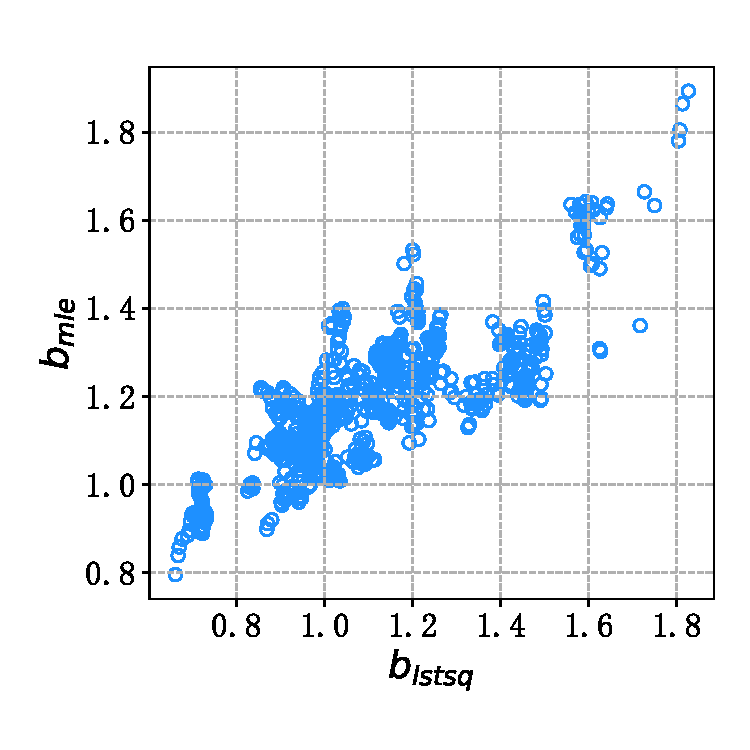
\includegraphics[width=0.50\textwidth]{Img/chap5_seism/seism_b_lstsq_mle_1932_2021.pdf}
  \vspace{-0.5cm}
  \bicaption[$b_\text{mle}$与$b_\text{lstsq}$]{$b_\text{mle}$与$b_\text{lstsq}$}{$b_\text{mle}$ and $b_\text{lstsq}$}
  \label{fig:seism_b_lstsq_mle_1932_2021}
\end{figure}

上节已经提到,$b$值的重要性和计算方法。图\ref{fig:seism_b_lstsq_mle_1932_2021}绘制了$b_\text{mle}$与$b_\text{lstsq}$关系图,发现两者的斜率接近于1。在获取$b$值后,也可得到其他几个与$b$值相关的地震因子,例如$a$值、最小二乘法的均方根误差$\eta$、最大震级欠缺$\Delta M$等。表\ref{tab:seism_input_data}描述了17个不同的地震因子,利用前16个因子作为输入预测最后1个因子。地震因子不仅包括\citet{Panakkat2007Neural}使用的最大震级$M_{\max}$、频度$\text{frequency}$、Giternberg-Richter法则中基于最小二乘法计算得到$a_{\text{lstsq}}$值、$b_{\text{lstsq}}$值、均方根误差$\eta$、最大震级欠缺$\Delta M$、最大似然估计法得到$b_{\text{mle}}$值、地震能量平方根$\sqrt{E}$和平均震级$M_{\text{mean}}$,还包括前人未曾使用的一些新特征。这些新特征包括平均纬度$\text{Lat}_{\text{mean}}$、纬度的均方根误差$\text{RMSE}_{\text{Lat}}$、平均经度$\text{Lon}_{\text{mean}}$、经度的均方根误差$\text{RMSE}_{\text{Lon}}$、按能量加权计算的震中平均纬度$\text{Lat}_{\sqrt{E}}$、按能量加权计算的震中平均经度$\text{Lon}_{\sqrt{E}}$、用最小二乘法计算的经纬度之间的斜率$k$,这7个地震因子能够体现地震发生的空间位置、地震成团或成带分布等。尽管部分因子在一定程度上高度相关,比如$M_{\text{mean}}$和$b_{\text{mle}}$,$b_{\text{mle}}$和$b_{\text{lstsq}}$,$M_{\max}$和$\sqrt{E}$,但研究时仍旧保留了这些冗余信息,因为机器学习不一定能够很好地捕获这些冗余信息。

\subsection{时空窗口滑动法}\label{sec:seism_slide}

第\ref{sec:ml_prepare}节已经介绍了窗口滑动法。在探索太阳黑子和泉流量时均采取了窗口滑动法,将原始观测数据集转化为监督学习数据集。与窗口滑动法有所差异,本章不仅在时间上对数据集进行滑动划分,在空间上也进行了同样的操作。这样做的目的是缩小预测震级的区域范围。因为研究不仅要关注震级,还要关注该震级发生的空间范围,而且该范围越小越好。

\begin{table}[htpb]
  \bicaption[每个时空窗口至少有30个地震数的时空窗口信息]{每个时空窗口至少有30个地震数的时空窗口信息。}{The time and space windows satisfy with 30 earthquake events at least 30.}
  \label{tab:seism_windows_30}
  \centering
  \footnotesize
  \begin{tabular}{cccc}
  \toprule
  \multirow{2}*{时间窗口} & \multirow{2}*{区块序号} & \multicolumn{2}{c}{空间窗口} \\
  \cmidrule(lr){3-4} \noalign{\smallskip}
  & & 纬度范围 & 经度范围 \\
  \midrule
  6年 & 1 & $[35.0N,37.0N]$ & $[114.0W,118.0W]$  \\
      & 2 &  $[35.0N,37.0N]$ & $[118.0W,122.0W]$  \\
      & 3 & $[33.5N,35.5]$ & $[114.0W,118.0W]$  \\
      & 4 & $[33.5N,35.5N]$ & $[117.5W,121.5W]$  \\
      & 5 & $[32.0N,34.0N]$ & $[114.0W,118.0W]$  \\
      & 6 & $[32.0N,34.0N]$ & $[117.0W,121.0W]$  \\
  \bottomrule
  \end{tabular} 
\end{table}

需要注意的是,部分地震因子的计算是基于统计学基础上的,因此每个时空窗口内地震数目需要达到某个值$N$。如果达不到该值,部分地震因子将会出现极端异常值。为了避免这种情况的出现,将每个时空窗口的地震数限制为至少30个。通常,7级以上的大震前兆会伴有半年至几年不等的前兆信息。因此,为了满足每个时空窗口的地震数至少为30,将时间窗口设为6年,空间窗口最小可设为纬度\SI{2}{\degree}\times 经度\SI{4}{\degree}。表\ref{tab:seism_windows_30}展示了每个时空窗口至少有30个地震数的时空窗口信息。

时间窗口按月滑动。空间窗口按照表\ref{tab:seism_windows_30}中区块序号进行滑动,即从研究区域的西北角开始向东滑动\SI{4}{\degree}。到达区域边缘后,再向南滑动\SI{1.5}{\degree}。向南滑动开始时离左边缘\SI{0.5}{\degree}向东滑动\SI{3.5}{\degree}。到达区域边缘后,再次向南滑动\SI{1.5}{\degree}。向南滑动开始时离左边缘\SI{1}{\degree}向东滑动\SI{3}{\degree}。这样重复几次后,一共得到6个空间区块。每次开始向南滑动时,西边的区块会右移,研究区域西南角为海域,地震目录中缺失了这部分的数据。根据时空窗口滑动,前16个地震因子和未来最大震级可被近似表达为:
\begin{equation}\adddotsbeforeeqnnum
  \label{eq:seism_m_indicator}
  \begin{split}
    M_{\text{future}}^{\text{loc}}(t+T)=F[M_{\text{max}}^{\text{loc}}(t-\Delta ),\text{frequency}^{\text{loc}}(t-\Delta ),M_{\text{mean}}^{\text{loc}}(t-\Delta ),\\
    b_{\text{lstsq}}^{\text{loc}}(t-\Delta ),b_{\text{mle}}^{\text{loc}}(t-\Delta ),a_{\text{lstsq}}^{\text{loc}}(t-\Delta ),\Delta^{\text{loc}}M(t-\Delta ),\\
    \sqrt{E}^{\text{loc}}(t-\Delta ),\eta^{\text{loc}}(t-\Delta ),\text{Lat}_{\text{mean}}^{\text{loc}}(t-\Delta ),\\
    \text{RMSE}_{\text{Lat}}^{\text{loc}}(t-\Delta ),\text{Lon}_{\text{mean}}^{\text{loc}}(t-\Delta ),\text{RMSE}_{\text{Lon}}^{\text{loc}}(t-\Delta ),
    \\
    \text{Lat}^{\text{loc}}_{\sqrt{E}}(t-\Delta),\text{Lon}^{\text{loc}}_{\sqrt{E}}(t-\Delta ),k^{\text{loc}}(t-\Delta),M_{\text{future}}^{\text{loc}}(t-\Delta)]
  \end{split}
\end{equation}
其中,$t$代表当前时刻,$-\Delta $代表历史时间窗口(即输入时间窗口),$+T$代表未来时间窗口(即输出时间窗口),$\text{loc}$代表区块序号,$\text{loc}\in\{1,2,\ldots,6\}$。$M_{\text{future}}^{\text{loc}}(t+T)$代表未来时间窗口$+T$内第$\text{loc}$个区块的最大震级。$M_{\text{max}}^{\text{loc}}(t- \Delta )$代表历史时间窗口$- \Delta $内第$\text{loc}$个区块的最大震级。其他变量的含义以此类推。

\section{结果分析}\label{sec:seism_result}

\subsection{基于6个区块预测未来1年的最大震级}\label{sec:seism_result_6}

\begin{figure}[!htbp]
  \centering
  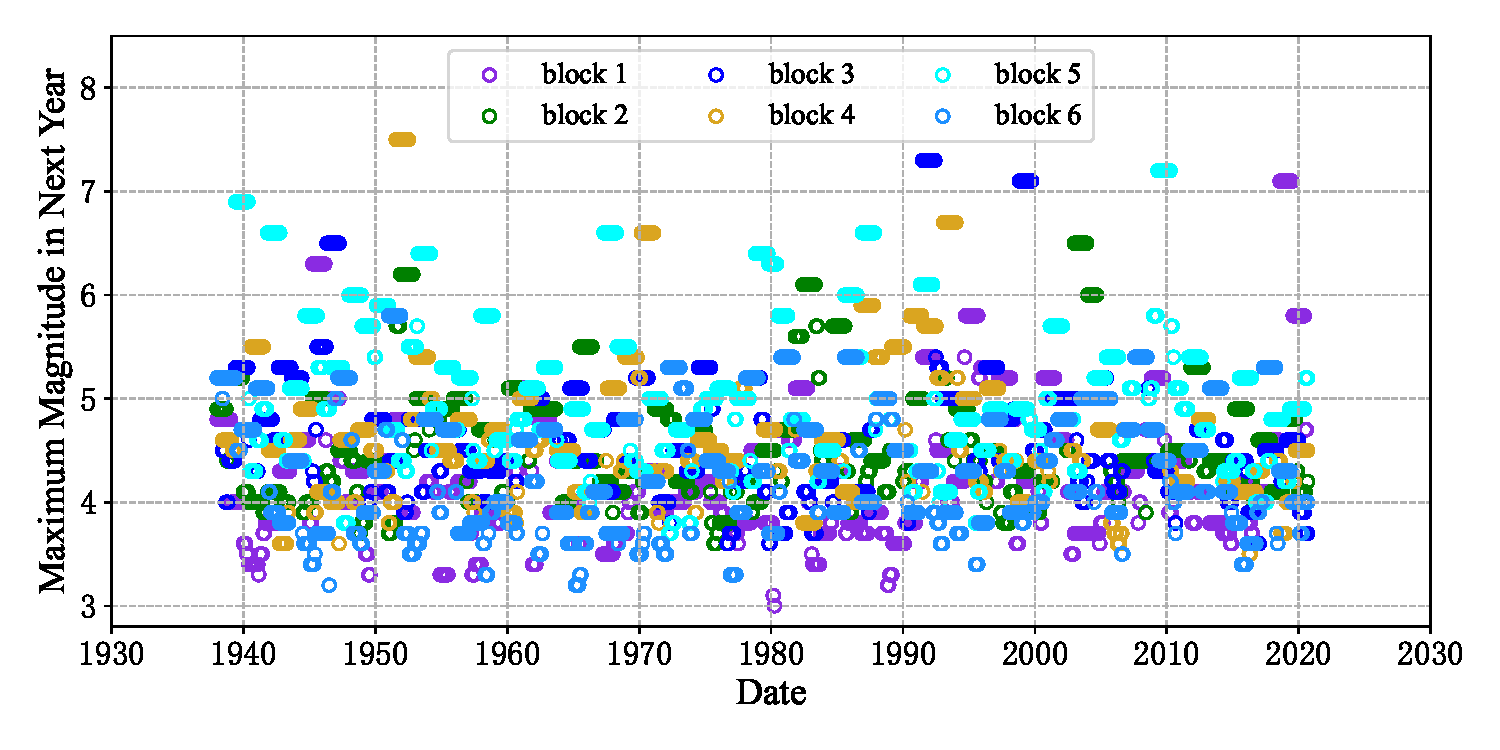
\includegraphics[width=\textwidth]{Img/chap5_seism/seism_magnitude_index_1932_2021.pdf}
  \vspace{-1cm}
  \bicaption[基于6个区块预测未来1年的最大震级]{基于6个区块预测未来1年的最大震级。}{The maximum magnitude in next year based on six blocks.}
  \label{fig:seism_magnitude_index_1932_2021}
\end{figure}

式\ref{eq:seism_m_indicator}明确指出,模型的输入是历史16个地震因子在6个不同区块的统计值,输出为未来时间窗口内的最大震级。图\ref{fig:seism_magnitude_index_1932_2021}绘制了不同区块未来1年最大震级时间序列图。从图\ref{fig:seism_magnitude_index_1932_2021}得知,该地区未来1年最大震级多数位于3.5至5.5之间。

这里采取了8种不同类型的模型,分别为LSTM-RNN、SVR、LR、RF、GBRT、DT、KNN、ETR。模型输入是6个区块在某个特定时刻前6年时间窗口内的16个地震因子,即输入为$6\times 16=96$个,输出是某个区块下一年的最大震级。数据集划分比例为0.8:0.2。针对两层的LSTM-RNN,第一层含32个LSTM神经元,最后一层为全连接层。训练经过1000回合,网络每层使用ReLU激活函数。批量训练数据量设为128。Adam方法作为优化器。学习率初始值设为$10^{-3}$。同时训练次数每增加10次,学习率会减小$1-10^{-6}$倍。所有试验均使用“早停”方案。

\begin{table}[!htbp]
  \bicaption[不同模型基于区块1预测未来1年最大震级的拟合指标效果(数据集划分比例为0.8:0.2)]{不同模型基于区块1预测未来1年最大震级的拟合指标效果(数据集划分比例为0.8:0.2)。}{The metrics for predicting the maximum magnitute of block 1 with the split ratio 0.8:0.2 in next year by different models.}
  \label{tab:seism_block1}
  \centering
  \footnotesize
  \begin{tabular}{lcccc}
    \toprule
    \multirow{2}*{模型} & \multicolumn{2}{c}{训练集} & \multicolumn{2}{c}{验证集} \\
    \cmidrule(lr){2-3} \cmidrule(lr){4-5} \noalign{\smallskip}
    & MSE & RMSE & MSE & RMSE \\
    \midrule
    LSTM & 0.0068 & 0.0826 & 0.0734 & 0.2710  \\
    SVR & 0.0069 & 0.0832 & 0.2116 & 0.4600  \\
    LR & 0.0054 & 0.0736 & 0.5800 & 0.7616  \\
    RF & 0.0014 & 0.0376 & 0.0452 & 0.2126  \\
    GBRT & 0.0012 & 0.0339 & 0.0663 & 0.2574  \\
    DT & \textbf{0.0000} & \textbf{0.0000} & 0.0558 & 0.2361  \\
    KNN & \textbf{0.0000} & \textbf{0.0000} & 0.0673 & 0.2595  \\
    ETR & \textbf{0.0000} & \textbf{0.0000} & 0.0778 & 0.2789  \\
    \bottomrule
  \end{tabular}
\end{table}

\begin{figure}[!htbp]
  \vspace{-2cm}
  \centering
  \begin{subfigure}[b]{0.45\textwidth}
    \caption{LSTM}
    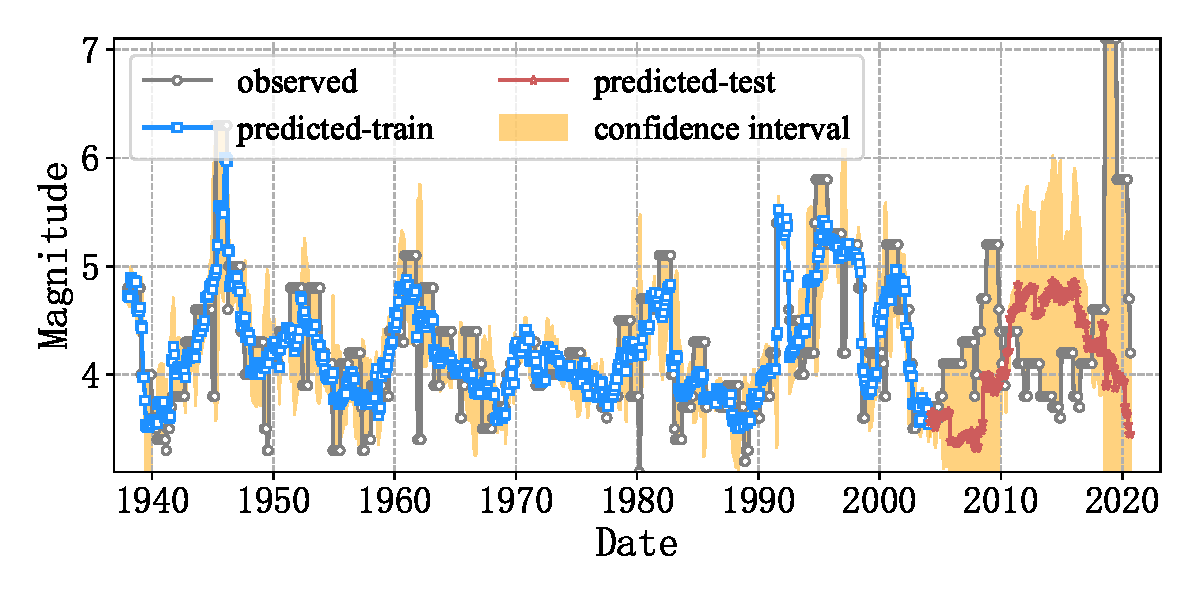
\includegraphics[width=\textwidth]{Img/chap5_seism/block1/seism_lstm_minyear_1932_maxyear_2021_spanlat_2_spanlon_4_timewindow_72_nextmonth_12_minmag_3.0_block_1.pdf}
    \vspace{-1cm}
    \label{fig:seism_lstm_minyear_1932_maxyear_2021_spanlat_2_spanlon_4_timewindow_72_nextmonth_12_minmag_3.0_block_1}
  \end{subfigure}
  ~
  \begin{subfigure}[b]{0.45\textwidth}
    \caption{SVR} 
    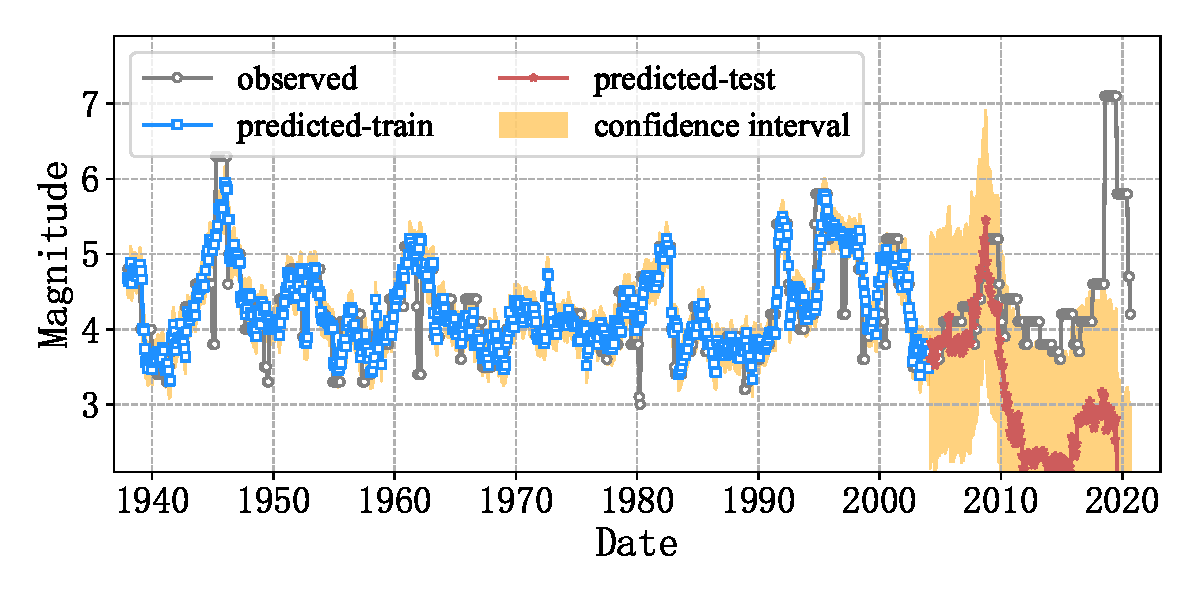
\includegraphics[width=\textwidth]{Img/chap5_seism/block1/seism_svr_minyear_1932_maxyear_2021_spanlat_2_spanlon_4_timewindow_72_nextmonth_12_minmag_3.0_block_1.pdf}
    \vspace{-1cm}
    \label{fig:seism_svr_minyear_1932_maxyear_2021_spanlat_2_spanlon_4_timewindow_72_nextmonth_12_minmag_3.0_block_1}
  \end{subfigure}   
  \\
  \begin{subfigure}[b]{0.45\textwidth}
      \caption{LR}
      \vspace{-0.2cm}
      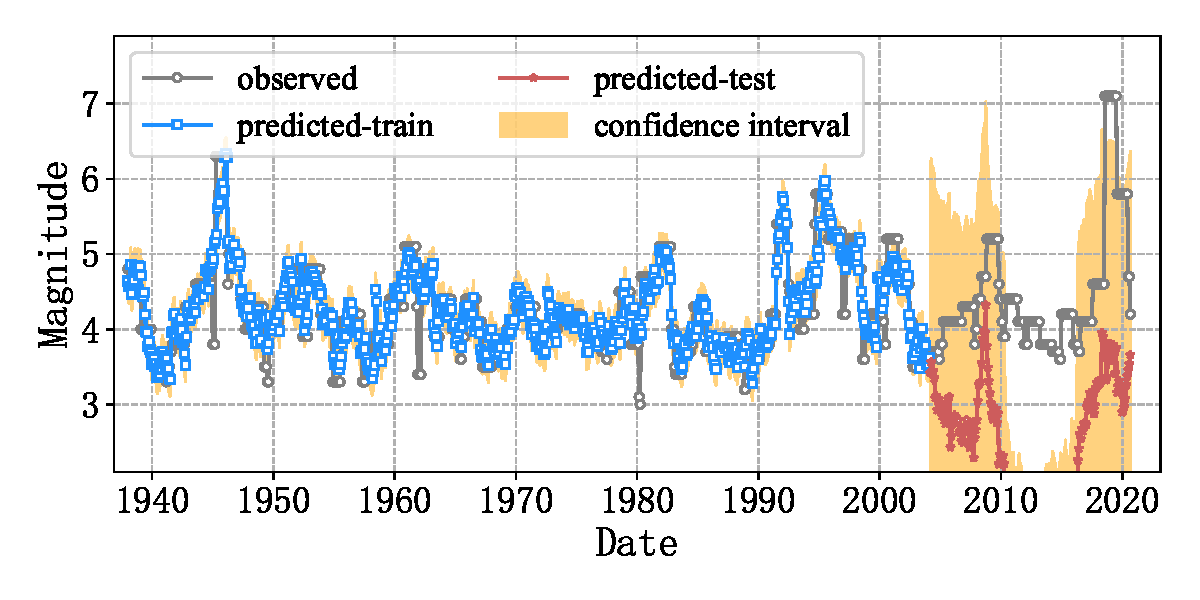
\includegraphics[width=\textwidth]{Img/chap5_seism/block1/seism_lr_minyear_1932_maxyear_2021_spanlat_2_spanlon_4_timewindow_72_nextmonth_12_minmag_3.0_block_1.pdf}
      \vspace{-1cm}
      \label{fig:seism_lr_minyear_1932_maxyear_2021_spanlat_2_spanlon_4_timewindow_72_nextmonth_12_minmag_3.0_block_1}
  \end{subfigure}
  ~
  \begin{subfigure}[b]{0.45\textwidth}
    \caption{RF}
    \vspace{-0.2cm}
    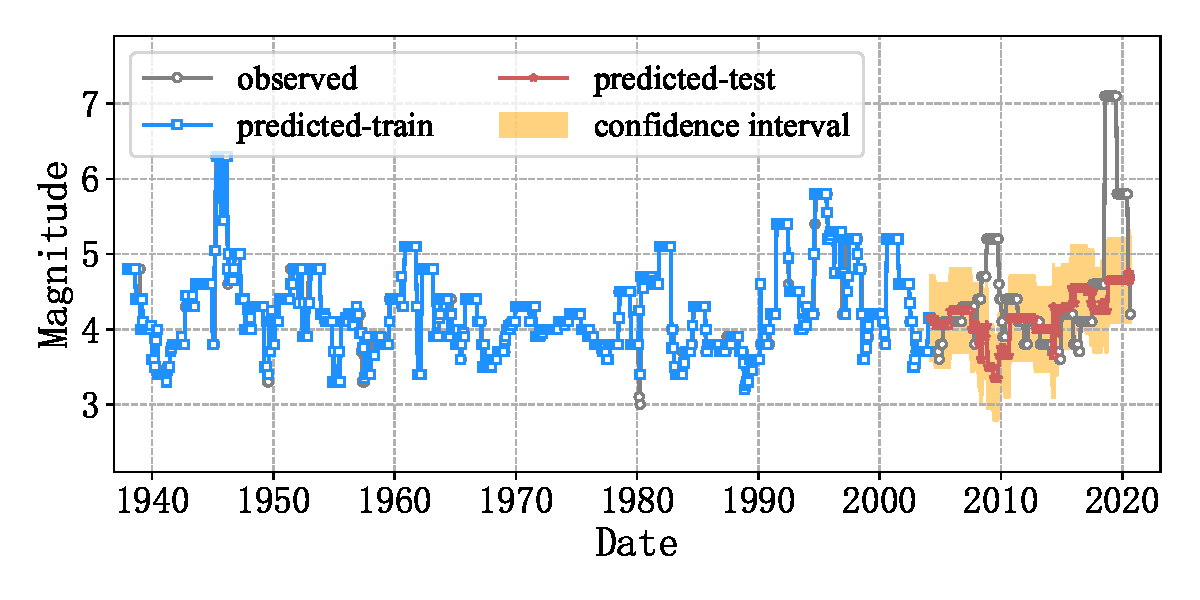
\includegraphics[width=\textwidth]{Img/chap5_seism/block1/seism_rf_minyear_1932_maxyear_2021_spanlat_2_spanlon_4_timewindow_72_nextmonth_12_minmag_3.0_block_1.pdf}
    \vspace{-1cm}
    \label{fig:seism_rf_minyear_1932_maxyear_2021_spanlat_2_spanlon_4_timewindow_72_nextmonth_12_minmag_3.0_block_1}
  \end{subfigure}
  \\
  \begin{subfigure}[b]{0.45\textwidth}
    \caption{GBRT}
    \vspace{-0.2cm}
    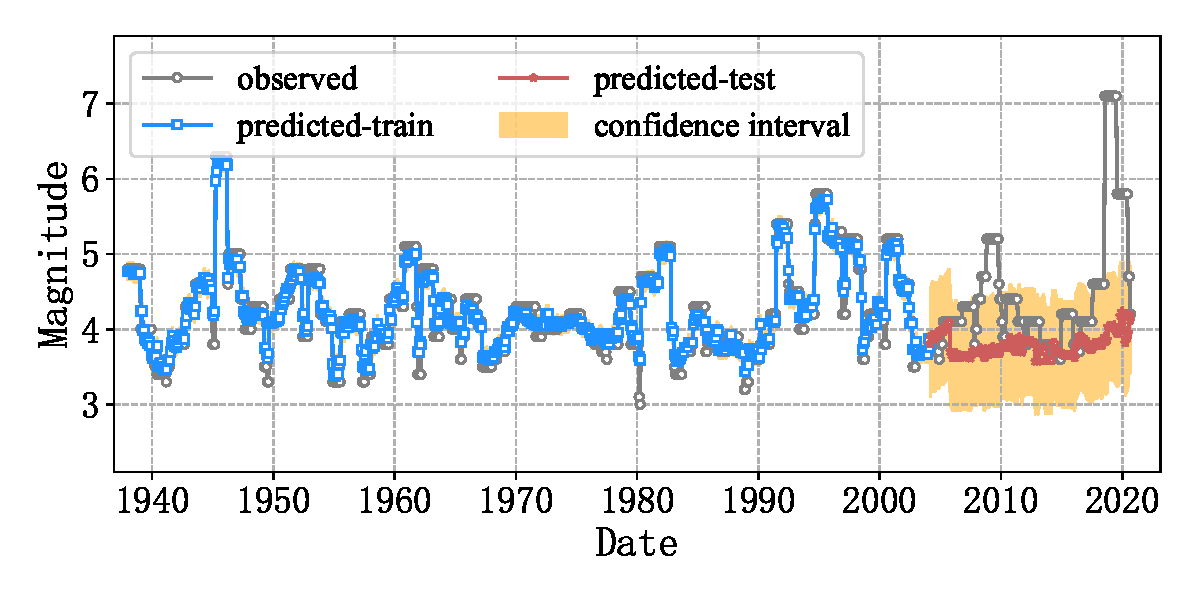
\includegraphics[width=\textwidth]{Img/chap5_seism/block1/seism_gbr_minyear_1932_maxyear_2021_spanlat_2_spanlon_4_timewindow_72_nextmonth_12_minmag_3.0_block_1.pdf}
    \vspace{-1cm}
    \label{fig:seism_gbr_minyear_1932_maxyear_2021_spanlat_2_spanlon_4_timewindow_72_nextmonth_12_minmag_3.0_block_1}
  \end{subfigure}
  ~
  \begin{subfigure}[b]{0.45\textwidth}
    \caption{DT}
    \vspace{-0.2cm}
    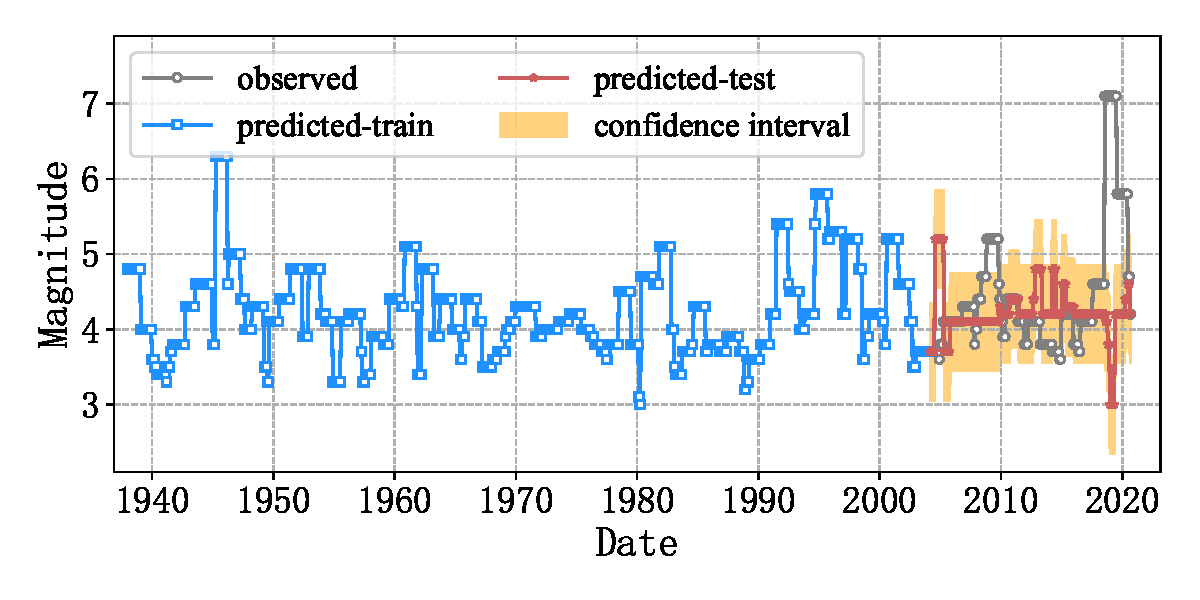
\includegraphics[width=\textwidth]{Img/chap5_seism/block1/seism_dt_minyear_1932_maxyear_2021_spanlat_2_spanlon_4_timewindow_72_nextmonth_12_minmag_3.0_block_1.pdf}
    \vspace{-1cm}
    \label{fig:seism_dt_minyear_1932_maxyear_2021_spanlat_2_spanlon_4_timewindow_72_nextmonth_12_minmag_3.0_block_1}
  \end{subfigure}
  \\
  \begin{subfigure}[b]{0.45\textwidth}
    \caption{KNN}
    \vspace{-0.2cm}
    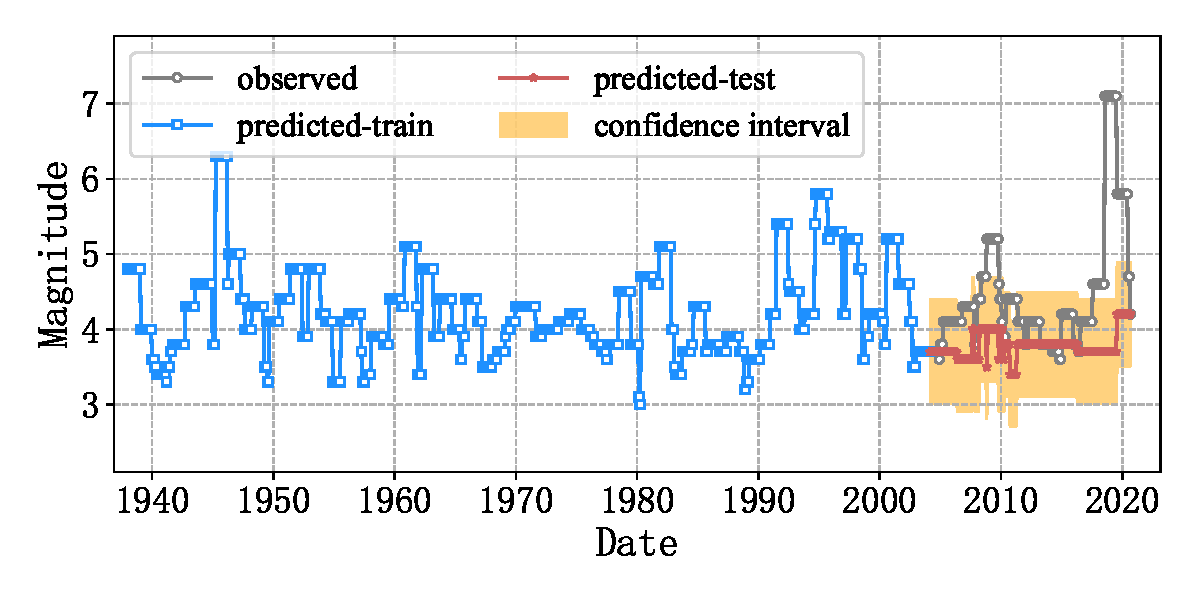
\includegraphics[width=\textwidth]{Img/chap5_seism/block1/seism_kn_minyear_1932_maxyear_2021_spanlat_2_spanlon_4_timewindow_72_nextmonth_12_minmag_3.0_block_1.pdf}
    \vspace{-1cm}
    \label{fig:seism_knn_minyear_1932_maxyear_2021_spanlat_2_spanlon_4_timewindow_72_nextmonth_12_minmag_3.0_block_1}
  \end{subfigure}
  ~
  \begin{subfigure}[b]{0.45\textwidth}
    \caption{ETR}
    \vspace{-0.2cm}
    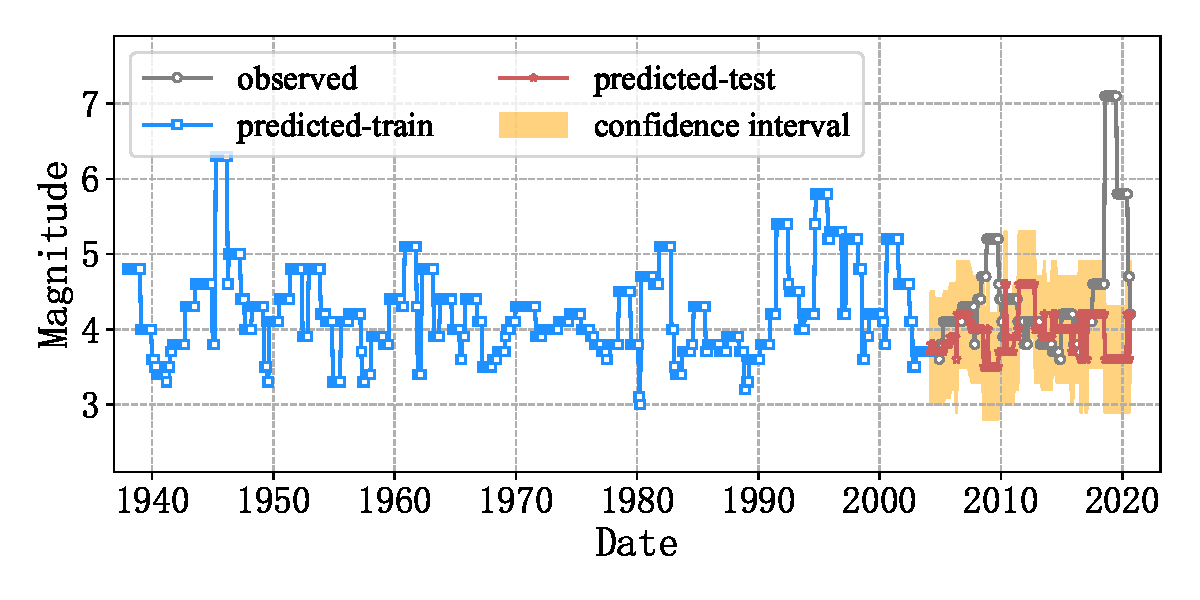
\includegraphics[width=\textwidth]{Img/chap5_seism/block1/seism_etr_minyear_1932_maxyear_2021_spanlat_2_spanlon_4_timewindow_72_nextmonth_12_minmag_3.0_block_1.pdf}
    \vspace{-1cm}
    \label{fig:seism_etr_minyear_1932_maxyear_2021_spanlat_2_spanlon_4_timewindow_72_nextmonth_12_minmag_3.0_block_1}
  \end{subfigure}
  \bicaption[不同模型基于区块1预测未来1年最大震级的时间序列图(数据集划分比例为0.8:0.2)]{不同模型基于区块1预测未来1年最大震级的时间序列图(数据集划分比例为0.8:0.2)。}{The time series of predicting the maximum magnitute  of block 1 with the split ratio 0.8:0.2 in next year by different models.}
  \label{fig:seism_minyear_1932_maxyear_2021_spanlat_2_spanlon_4_timewindow_72_nextmonth_12_minmag_3.0_block_1}
\end{figure}

将区块分成6个子任务进行试验。区块2-6的试验结果被放在了附录中(见第\ref{sec:seis_table_figure}节)。表\ref{tab:seism_block1}和表\ref{tab:seism_block}中展示了6个不同区块在不同模型下预报未来1年最大震级的拟合指标效果。图\ref{fig:seism_minyear_1932_maxyear_2021_spanlat_2_spanlon_4_timewindow_72_nextmonth_12_minmag_3.0_block_1}至图\ref{fig:seism_minyear_1932_maxyear_2021_spanlat_2_spanlon_4_timewindow_72_nextmonth_12_minmag_3.0_block_6}展示了6个不同区块拟合未来1年最大震级的时间序列,横轴时间$t$代表着未来$[t,t+1]$年时间段内的最大震级。由表\ref{tab:seism_block1}和表\ref{tab:seism_block}、图\ref{fig:seism_minyear_1932_maxyear_2021_spanlat_2_spanlon_4_timewindow_72_nextmonth_12_minmag_3.0_block_1}至图\ref{fig:seism_minyear_1932_maxyear_2021_spanlat_2_spanlon_4_timewindow_72_nextmonth_12_minmag_3.0_block_6}可知,两层的LSTM-RNN、SVR、LR、RF、GBRT、DT、KNN、ETR均出现了很大程度的过拟合现象。对于DT、KNN、ETR这三种机器学习模型,甚至能够拟合全部的训练集,而对测试集却无能为力。机器学习相对于本数据集而言,过于复杂,因此机器学习对南加州地区的地震中期预报是失败的。

\subsection{基于整个区块预测未来1年的最大震级}\label{sec:seism_result_1}

鉴于第\ref{sec:seism_result_6}节的结果,这里试图不对区域进行划分滑动,采用滑动窗口法获取模型的输入和输出。同样采取了8种不同类型的模型。模型输入是整个区块在某个特定时刻前6年时间窗口内16个预报因子,即输入为$16$个,输出是整个区块下一年的最大震级。数据集划分比例为0.8:0.2。LSTM-RNN网络的设置和超参数的使用同上。

\begin{table}[!htbp]
  \bicaption[不同模型基于整个区块预测未来1年最大震级的拟合指标效果(数据集划分比例为0.8:0.2)]{不同模型基于整个区块预测未来1年最大震级的拟合指标效果(数据集划分比例为0.8:0.2)。}{The metrics for predicting the maximum magnitute with the split ratio 0.8:0.2 in next year by different models.}
  \label{tab:seism_minyear_1932_maxyear_2021_spanlat_2_spanlon_4_timewindow_72_nextmonth_12_minmag_3.0_blocks1}
  \centering
  \footnotesize
  \begin{tabular}{lcccc}
    \toprule
    \multirow{2}*{模型} & \multicolumn{2}{c}{训练集} & \multicolumn{2}{c}{验证集} \\
    \cmidrule(lr){2-3} \cmidrule(lr){4-5} \noalign{\smallskip}
    & MSE & RMSE & MSE & RMSE \\
    \midrule
    LSTM & 0.0367 & 0.1916 & 0.0444 & 0.2108 \\
    SVR & 0.0396 & 0.1989 & 0.0453 & 0.2127 \\
    LR & 0.0349 & 0.1868 & 0.0636 & 0.2522 \\
    RF & 0.0026 & 0.0511 & 0.0433 & 0.2082 \\
    GBRT & 0.0053 & 0.0728 & 0.0451 & 0.2125 \\
    DT & \textbf{0.0000} & \textbf{0.0000} & 0.0767 & 0.2770 \\
    KNN & \textbf{0.0000} & \textbf{0.0000} & 0.1603 & 0.4004 \\
    ETR & \textbf{0.0000} & \textbf{0.0000} & 0.1457 & 0.3817 \\
    \bottomrule
  \end{tabular}
\end{table}

\begin{figure}[!htbp]
  \centering
  \begin{subfigure}[b]{0.45\textwidth}
    \caption{LSTM}
    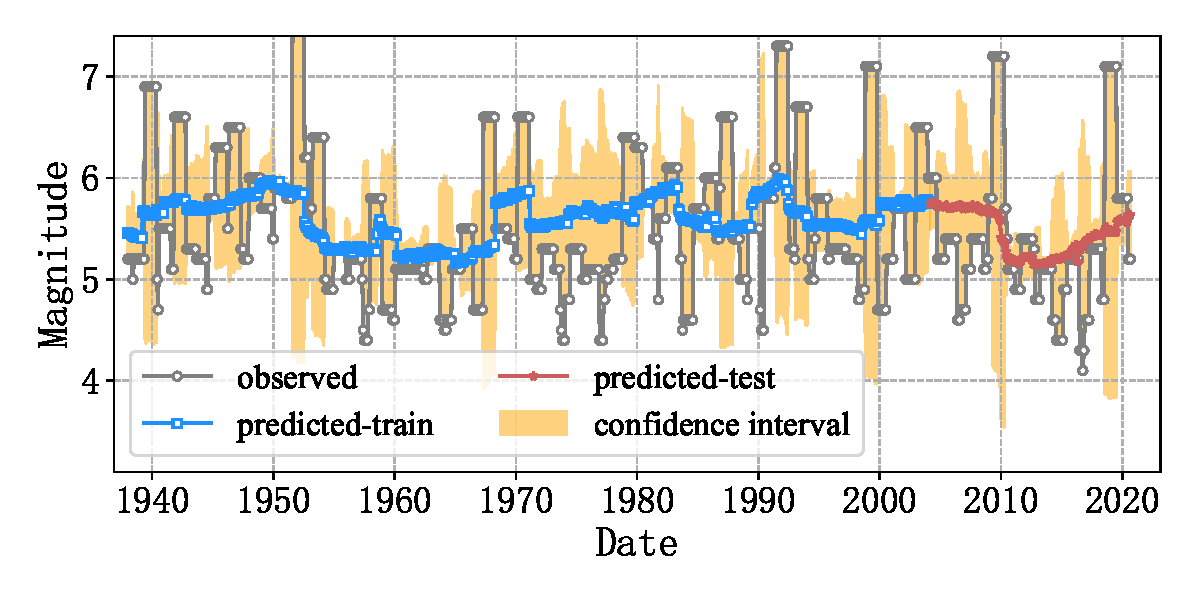
\includegraphics[width=\textwidth]{Img/chap5_seism/total/seism_lstm_minyear_1932_maxyear_2021_spanlat_2_spanlon_4_timewindow_72_nextmonth_12_minmag_3.0_blocks1.pdf}
    \vspace{-1cm}
    \label{fig:seism_lstm_minyear_1932_maxyear_2021_spanlat_2_spanlon_4_timewindow_72_nextmonth_12_minmag_3.0_blocks1}
  \end{subfigure}
  ~
  \begin{subfigure}[b]{0.45\textwidth}
    \caption{SVR} 
    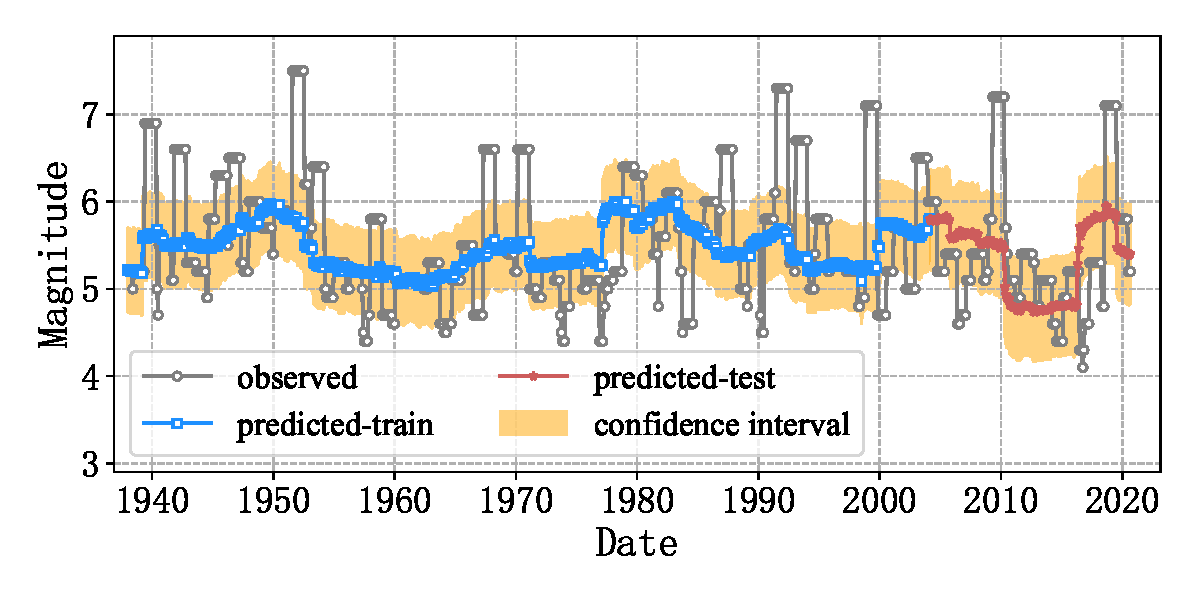
\includegraphics[width=\textwidth]{Img/chap5_seism/total/seism_svr_minyear_1932_maxyear_2021_spanlat_2_spanlon_4_timewindow_72_nextmonth_12_minmag_3.0_blocks1.pdf}
    \vspace{-1cm}
    \label{fig:seism_svr_minyear_1932_maxyear_2021_spanlat_2_spanlon_4_timewindow_72_nextmonth_12_minmag_3.0_blocks1}
  \end{subfigure}   
  \\
  \begin{subfigure}[b]{0.45\textwidth}
      \caption{LR}
      \vspace{-0.2cm}
      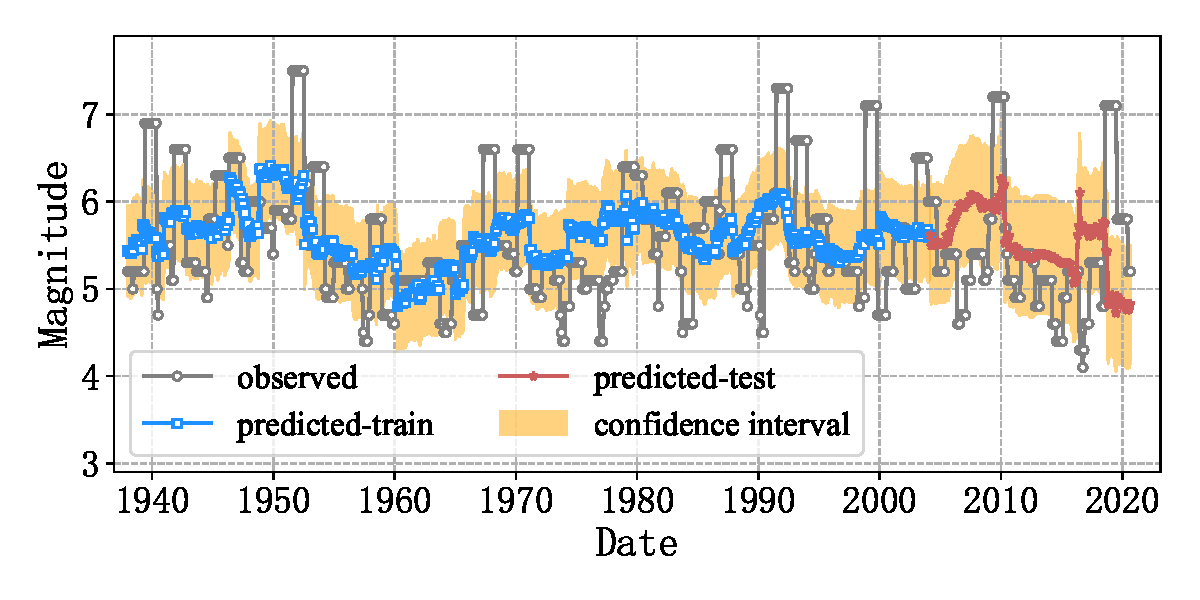
\includegraphics[width=\textwidth]{Img/chap5_seism/total/seism_lr_minyear_1932_maxyear_2021_spanlat_2_spanlon_4_timewindow_72_nextmonth_12_minmag_3.0_blocks1.pdf}
      \vspace{-1cm}
      \label{fig:seism_lr_minyear_1932_maxyear_2021_spanlat_2_spanlon_4_timewindow_72_nextmonth_12_minmag_3.0_blocks1}
  \end{subfigure}
  ~
  \begin{subfigure}[b]{0.45\textwidth}
    \caption{RF}
    \vspace{-0.2cm}
    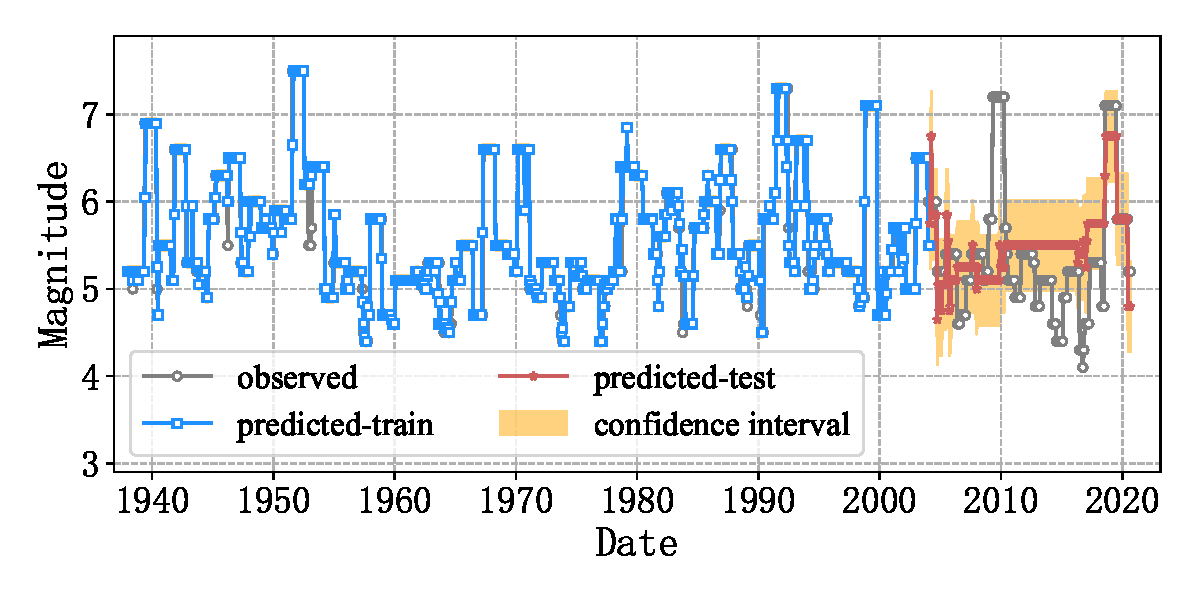
\includegraphics[width=\textwidth]{Img/chap5_seism/total/seism_rf_minyear_1932_maxyear_2021_spanlat_2_spanlon_4_timewindow_72_nextmonth_12_minmag_3.0_blocks1.pdf}
    \vspace{-1cm}
    \label{fig:seism_rf_minyear_1932_maxyear_2021_spanlat_2_spanlon_4_timewindow_72_nextmonth_12_minmag_3.0_blocks1}
  \end{subfigure}
  \\
  \begin{subfigure}[b]{0.45\textwidth}
    \caption{GBRT}
    \vspace{-0.2cm}
    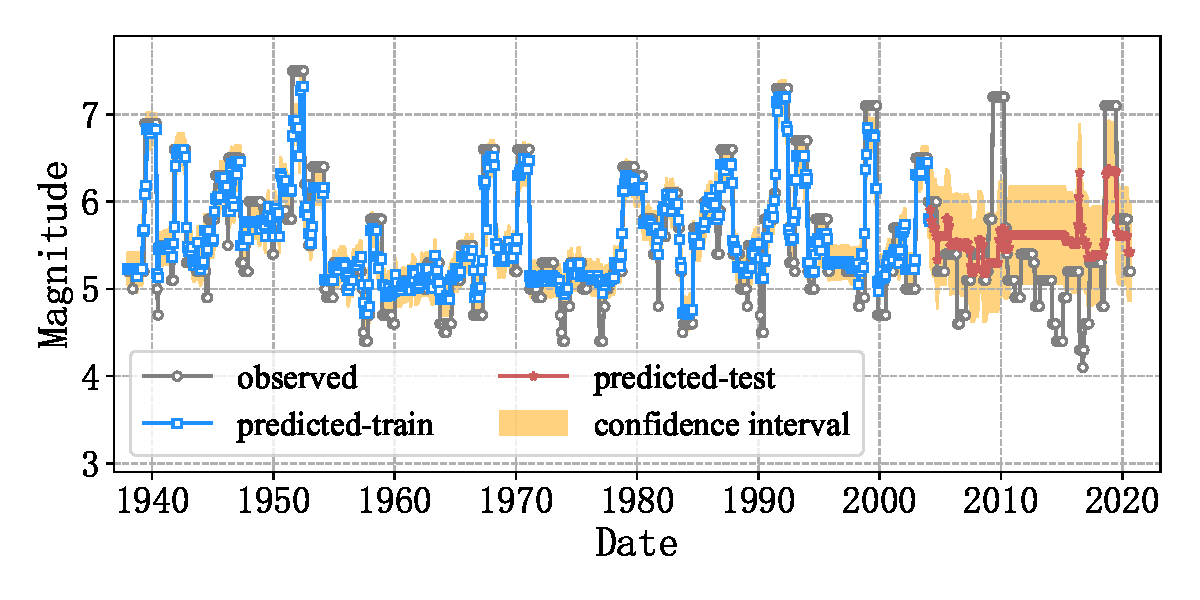
\includegraphics[width=\textwidth]{Img/chap5_seism/total/seism_gbr_minyear_1932_maxyear_2021_spanlat_2_spanlon_4_timewindow_72_nextmonth_12_minmag_3.0_blocks1.pdf}
    \vspace{-1cm}
    \label{fig:seism_gbr_minyear_1932_maxyear_2021_spanlat_2_spanlon_4_timewindow_72_nextmonth_12_minmag_3.0_blocks1}
  \end{subfigure}
  ~
  \begin{subfigure}[b]{0.45\textwidth}
    \caption{DT}
    \vspace{-0.2cm}
    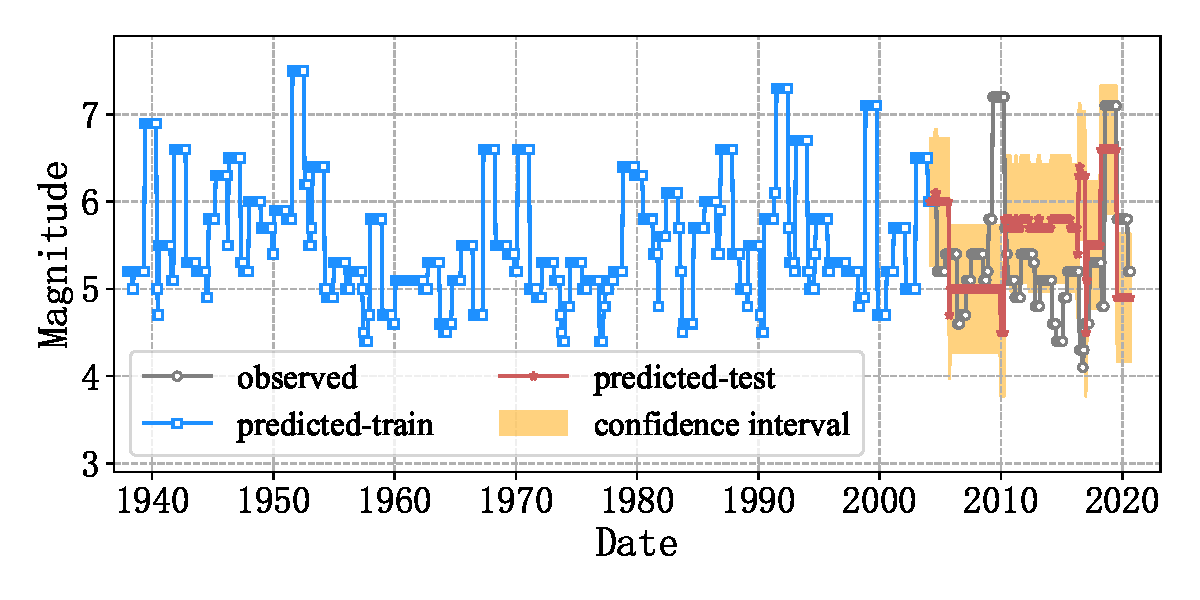
\includegraphics[width=\textwidth]{Img/chap5_seism/total/seism_dt_minyear_1932_maxyear_2021_spanlat_2_spanlon_4_timewindow_72_nextmonth_12_minmag_3.0_blocks1.pdf}
    \vspace{-1cm}
    \label{fig:seism_dt_minyear_1932_maxyear_2021_spanlat_2_spanlon_4_timewindow_72_nextmonth_12_minmag_3.0_blocks1}
  \end{subfigure}
  \\
  \begin{subfigure}[b]{0.45\textwidth}
    \caption{KNN}
    \vspace{-0.2cm}
    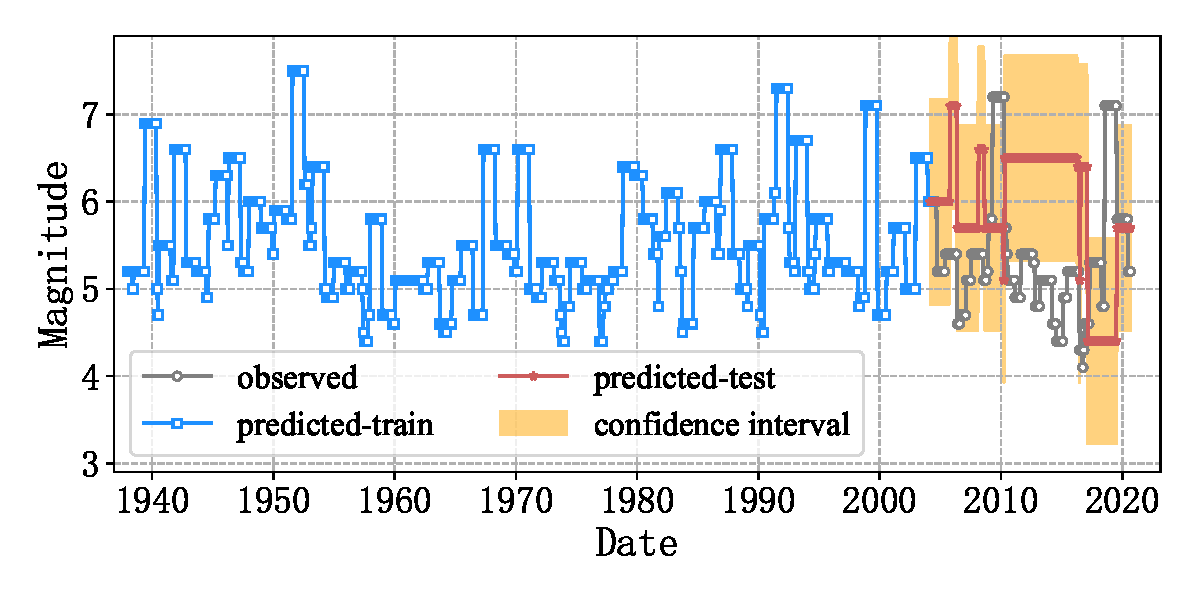
\includegraphics[width=\textwidth]{Img/chap5_seism/total/seism_kn_minyear_1932_maxyear_2021_spanlat_2_spanlon_4_timewindow_72_nextmonth_12_minmag_3.0_blocks1.pdf}
    \vspace{-1cm}
    \label{fig:seism_knn_minyear_1932_maxyear_2021_spanlat_2_spanlon_4_timewindow_72_nextmonth_12_minmag_3.0_blocks1}
  \end{subfigure}
  ~
  \begin{subfigure}[b]{0.45\textwidth}
    \caption{ETR}
    \vspace{-0.2cm}
    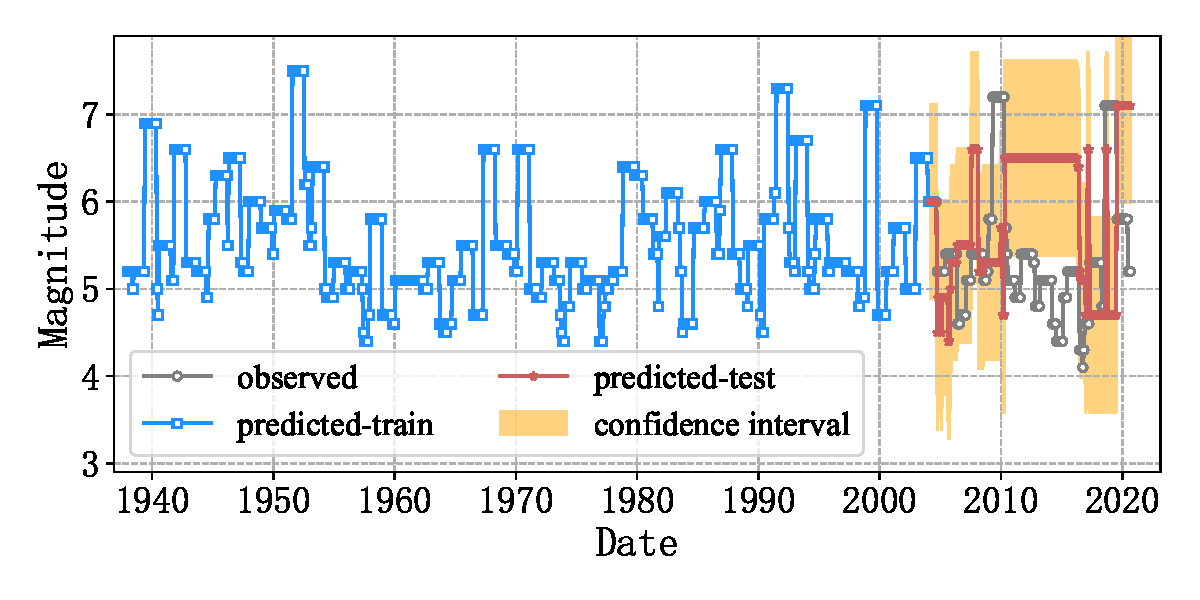
\includegraphics[width=\textwidth]{Img/chap5_seism/total/seism_etr_minyear_1932_maxyear_2021_spanlat_2_spanlon_4_timewindow_72_nextmonth_12_minmag_3.0_blocks1.pdf}
    \vspace{-1cm}
    \label{fig:seism_etr_minyear_1932_maxyear_2021_spanlat_2_spanlon_4_timewindow_72_nextmonth_12_minmag_3.0_blocks1}
  \end{subfigure}
  \bicaption[不同模型基于整个区块预测未来1年最大震级的时间序列图(数据集划分比例为0.8:0.2)]{不同模型基于整个区块预测未来1年最大震级的时间序列图(数据集划分比例为0.8:0.2)。}{The time series of predicting the maximum magnitute with the split ratio 0.8:0.2 in next year by different models.}
  \label{fig:seism_minyear_1932_maxyear_2021_spanlat_2_spanlon_4_timewindow_72_nextmonth_12_minmag_3.0_blocks1}
\end{figure}

表\ref{tab:seism_minyear_1932_maxyear_2021_spanlat_2_spanlon_4_timewindow_72_nextmonth_12_minmag_3.0_blocks1}展示了整个区块在不同模型下预报未来1年最大震级的拟合指标效果。图\ref{fig:seism_minyear_1932_maxyear_2021_spanlat_2_spanlon_4_timewindow_72_nextmonth_12_minmag_3.0_blocks1}展示了整个区块拟合未来1年最大震级的时间序列,横轴时间$t$代表着未来$[t,t+1]$年时间段内的最大震级。
由表\ref{tab:seism_minyear_1932_maxyear_2021_spanlat_2_spanlon_4_timewindow_72_nextmonth_12_minmag_3.0_blocks1}和图\ref{fig:seism_minyear_1932_maxyear_2021_spanlat_2_spanlon_4_timewindow_72_nextmonth_12_minmag_3.0_blocks1}可知,几种模型仍均出现了很大程度的过拟合现象。同第\ref{sec:seism_result_1}节的结论,机器学习对南加州地区的地震中期预报是失败的。

\subsection{基于整个区块预测未来10年的最大震级}\label{sec:seism_result_10}

\subsubsection{验证集:测试集=0.8:0.2}\label{sec:seism_result_10_80}

鉴于第\ref{sec:seism_result_1}节的结果,这里试图延长输出时间窗口,即预测未来10年的最大震级。同样采取了8种不同类型的模型。模型输入是整个区块在某个特定时刻前10年时间窗口内的16个预报因子,即输入为$16$个,输出是整个区块未来10年的最大震级。数据集划分比例为0.8:0.2。LSTM-RNN网络的设置和超参数的使用同上。

\begin{table}[!htbp]
  \bicaption[不同模型基于整个区块预测未来10年最大震级的拟合指标效果(数据集划分比例为0.8:0.2)]{不同模型基于整个区块预测未来10年最大震级的拟合指标效果(数据集划分比例为0.8:0.2)。}{The metrics for predicting the maximum magnitute with the split ratio 0.8:0.2 in next ten years by different models.}
  \label{tab:seism_minyear_1932_maxyear_2021_spanlat_2_spanlon_4_timewindow_120_nextmonth_120_minmag_3.0_blocks1}
  \centering
  \footnotesize
  \begin{tabular}{lcccc}
    \toprule
    \multirow{2}*{模型} & \multicolumn{2}{c}{训练集} & \multicolumn{2}{c}{验证集} \\
    \cmidrule(lr){2-3} \cmidrule(lr){4-5} \noalign{\smallskip}
    & MSE & RMSE & MSE & RMSE \\
    \midrule
    LSTM & 0.0127 & 0.1125 & 0.0409 & 0.2021 \\
    SVR & 0.0207 & 0.1439 & 0.0164 & 0.1280 \\
    LR & 0.0114 & 0.1067 & 0.0320 & 0.1789 \\
    RF & 0.0004 & 0.0201 & 0.1288 & 0.3589 \\
    GBRT & 0.0001 & 0.0099 & 0.2016 & 0.4490 \\
    DT & \textbf{0.0000} & \textbf{0.0000} & 0.2668 & 0.5165 \\
    KNN & \textbf{0.0000} & \textbf{0.0000} & 0.0265 & 0.1627 \\
    ETR & \textbf{0.0000} & \textbf{0.0000} & 0.2285 & 0.4781 \\
    \bottomrule
  \end{tabular}
\end{table}

\begin{figure}[!htbp]
  \vspace{-2cm}
  \centering
  \begin{subfigure}[b]{0.45\textwidth}
    \caption{LSTM}
    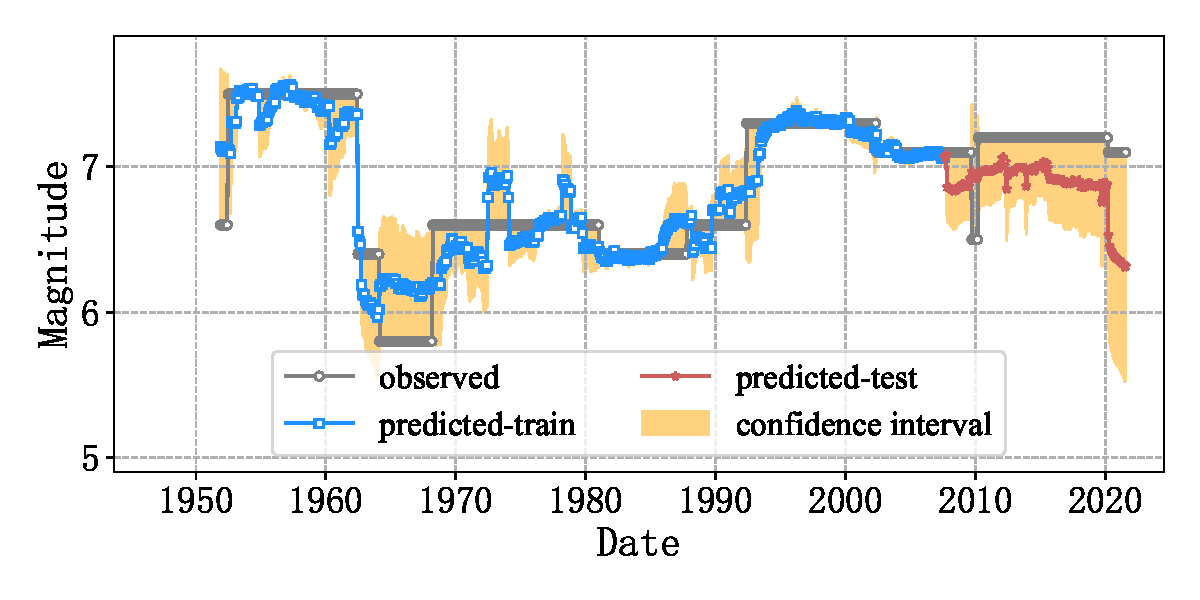
\includegraphics[width=\textwidth]{Img/chap5_seism/future10/seism_lstm_minyear_1932_maxyear_2021_spanlat_2_spanlon_4_timewindow_120_nextmonth_120_minmag_3.0_blocks1.pdf}
    \vspace{-1cm}
    \label{fig:seism_lstm_minyear_1932_maxyear_2021_spanlat_2_spanlon_4_timewindow_120_nextmonth_120_minmag_3.0_blocks1}
  \end{subfigure}
  ~
  \begin{subfigure}[b]{0.45\textwidth}
    \caption{SVR} 
    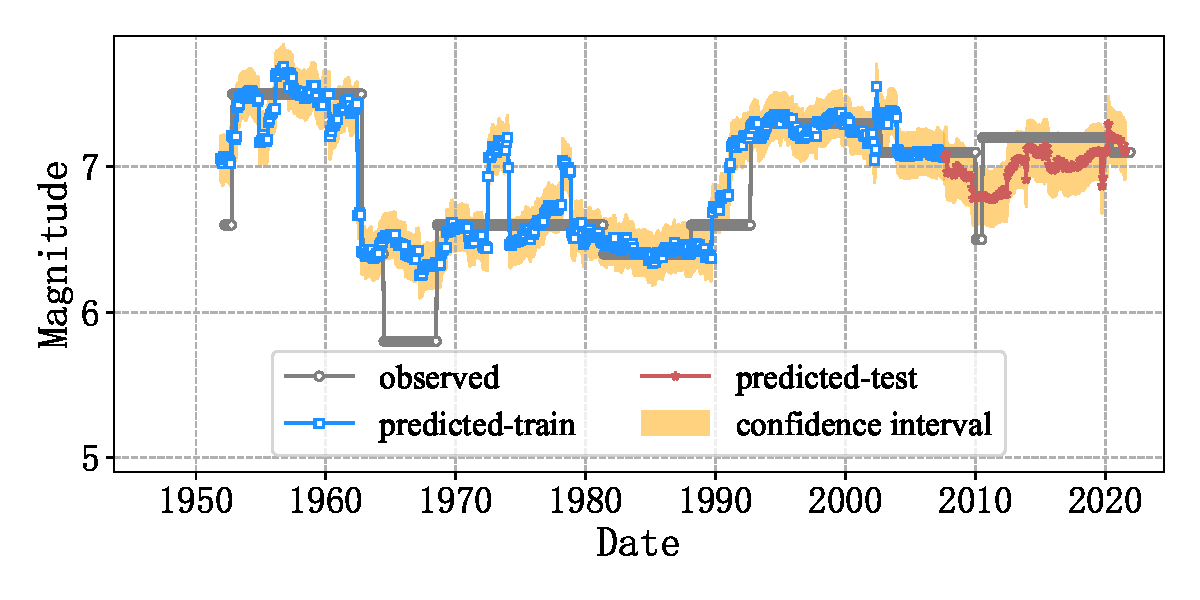
\includegraphics[width=\textwidth]{Img/chap5_seism/future10/seism_svr_minyear_1932_maxyear_2021_spanlat_2_spanlon_4_timewindow_120_nextmonth_120_minmag_3.0_blocks1.pdf}
    \vspace{-1cm}
    \label{fig:seism_svr_minyear_1932_maxyear_2021_spanlat_2_spanlon_4_timewindow_120_nextmonth_120_minmag_3.0_blocks1}
  \end{subfigure}   
  \\
  \begin{subfigure}[b]{0.45\textwidth}
      \caption{LR}
      \vspace{-0.2cm}
      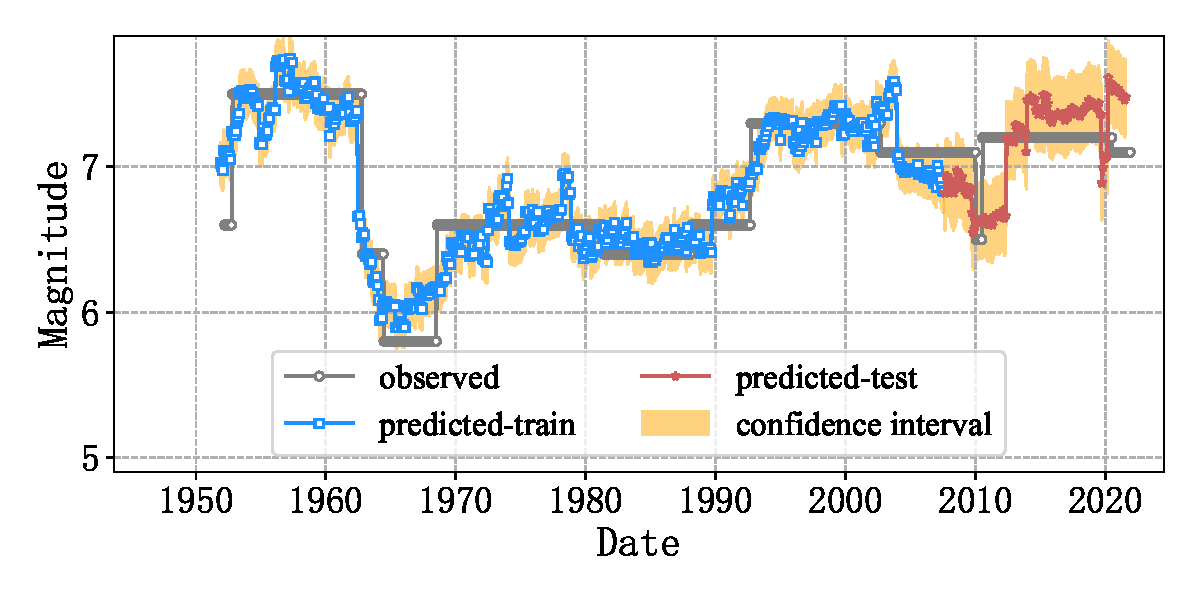
\includegraphics[width=\textwidth]{Img/chap5_seism/future10/seism_lr_minyear_1932_maxyear_2021_spanlat_2_spanlon_4_timewindow_120_nextmonth_120_minmag_3.0_blocks1.pdf}
      \vspace{-1cm}
      \label{fig:seism_lr_minyear_1932_maxyear_2021_spanlat_2_spanlon_4_timewindow_120_nextmonth_120_minmag_3.0_blocks1}
  \end{subfigure}
  ~
  \begin{subfigure}[b]{0.45\textwidth}
    \caption{RF}
    \vspace{-0.2cm}
    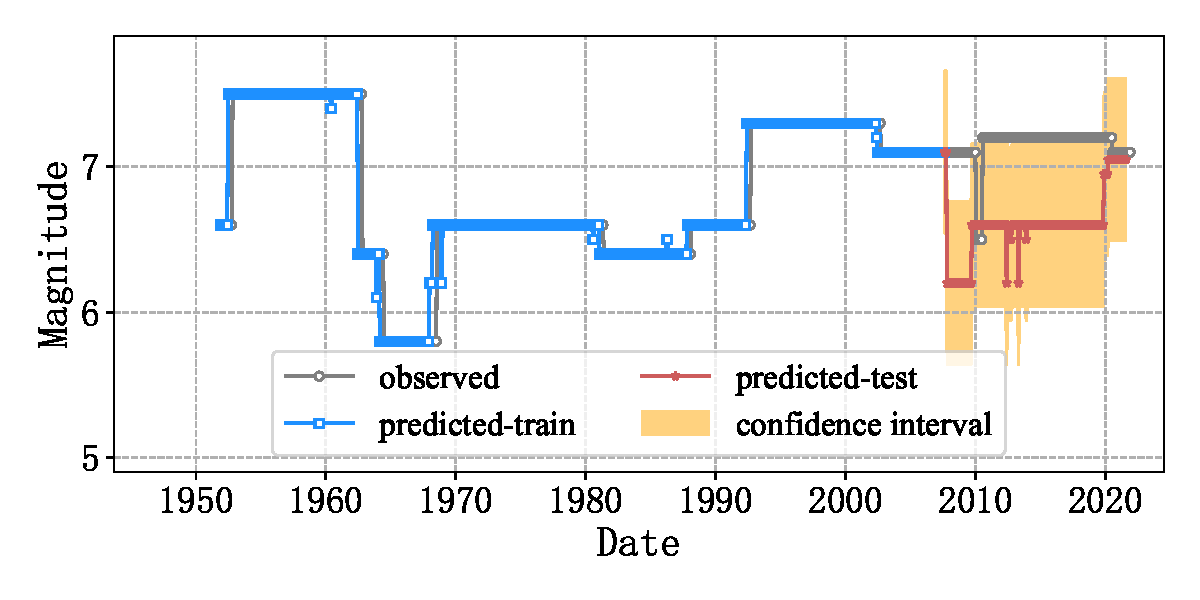
\includegraphics[width=\textwidth]{Img/chap5_seism/future10/seism_rf_minyear_1932_maxyear_2021_spanlat_2_spanlon_4_timewindow_120_nextmonth_120_minmag_3.0_blocks1.pdf}
    \vspace{-1cm}
    \label{fig:seism_rf_minyear_1932_maxyear_2021_spanlat_2_spanlon_4_timewindow_120_nextmonth_120_minmag_3.0_blocks1}
  \end{subfigure}
  \\
  \begin{subfigure}[b]{0.45\textwidth}
    \caption{GBRT}
    \vspace{-0.2cm}
    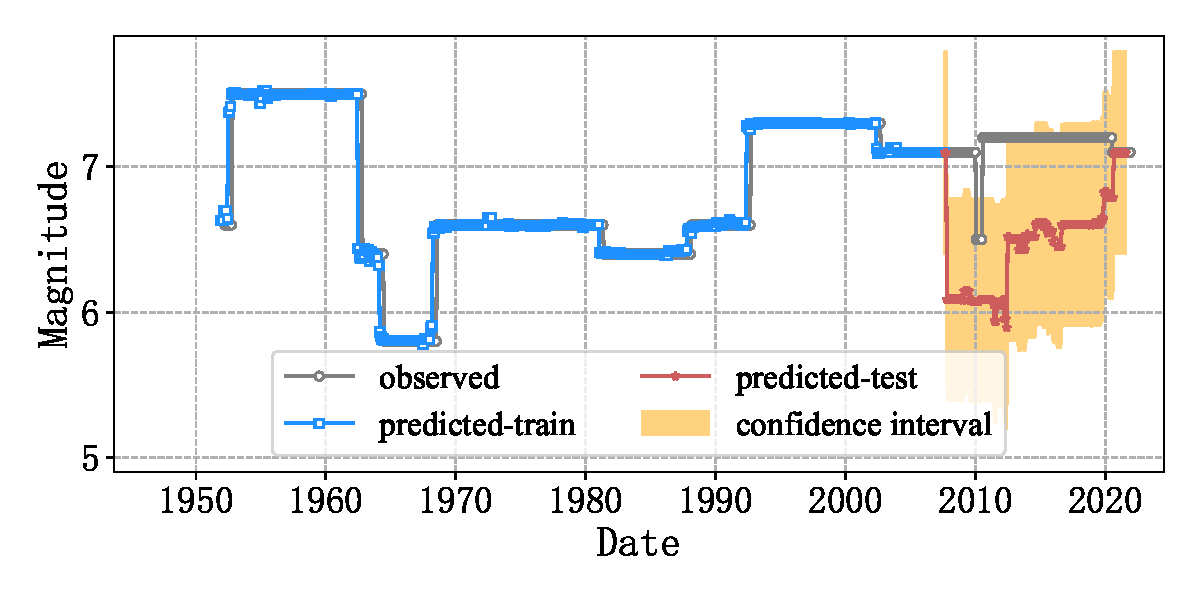
\includegraphics[width=\textwidth]{Img/chap5_seism/future10/seism_gbr_minyear_1932_maxyear_2021_spanlat_2_spanlon_4_timewindow_120_nextmonth_120_minmag_3.0_blocks1.pdf}
    \vspace{-1cm}
    \label{fig:seism_gbr_minyear_1932_maxyear_2021_spanlat_2_spanlon_4_timewindow_120_nextmonth_120_minmag_3.0_blocks1}
  \end{subfigure}
  ~
  \begin{subfigure}[b]{0.45\textwidth}
    \caption{DT}
    \vspace{-0.2cm}
    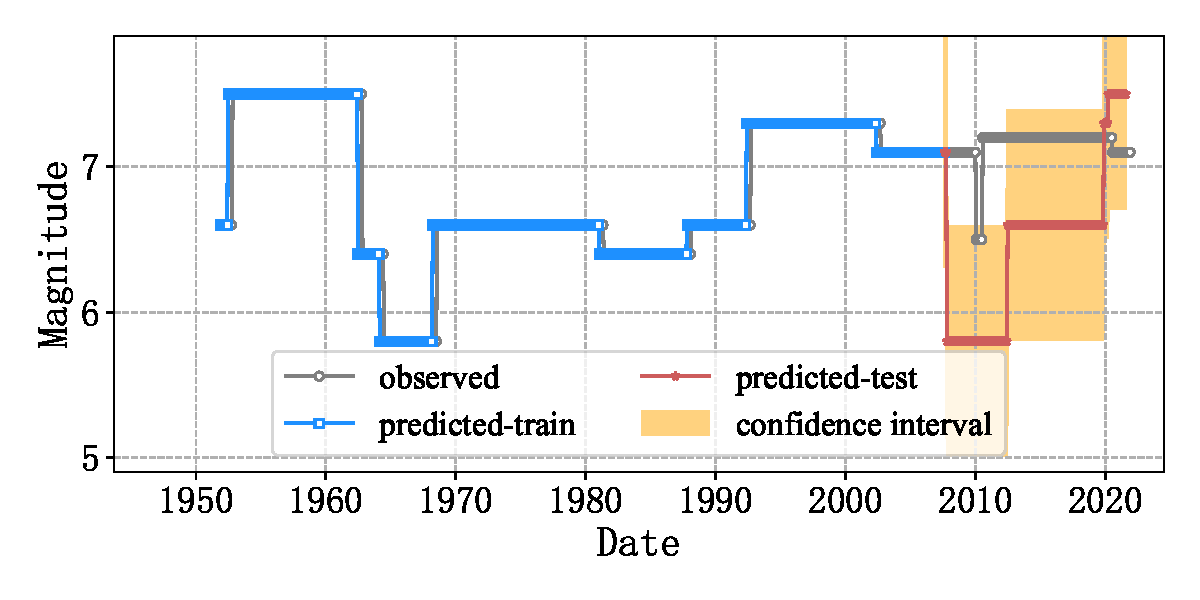
\includegraphics[width=\textwidth]{Img/chap5_seism/future10/seism_dt_minyear_1932_maxyear_2021_spanlat_2_spanlon_4_timewindow_120_nextmonth_120_minmag_3.0_blocks1.pdf}
    \vspace{-1cm}
    \label{fig:seism_dt_minyear_1932_maxyear_2021_spanlat_2_spanlon_4_timewindow_120_nextmonth_120_minmag_3.0_blocks1}
  \end{subfigure}
  \\
  \begin{subfigure}[b]{0.45\textwidth}
    \caption{KNN}
    \vspace{-0.2cm}
    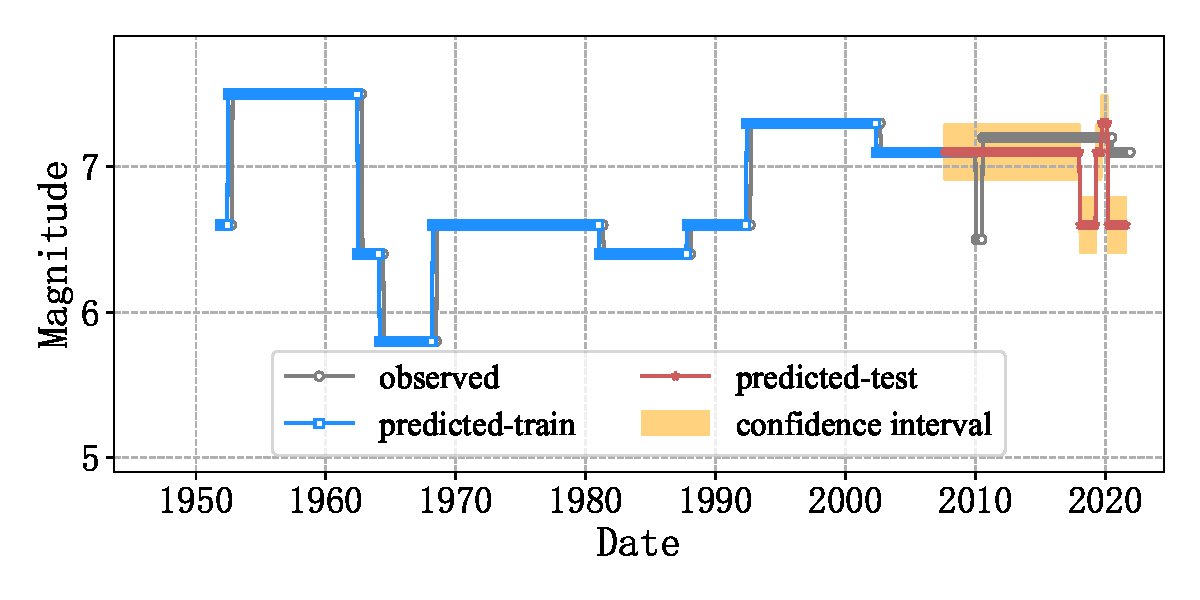
\includegraphics[width=\textwidth]{Img/chap5_seism/future10/seism_kn_minyear_1932_maxyear_2021_spanlat_2_spanlon_4_timewindow_120_nextmonth_120_minmag_3.0_blocks1.pdf}
    \vspace{-1cm}
    \label{fig:seism_knn_minyear_1932_maxyear_2021_spanlat_2_spanlon_4_timewindow_120_nextmonth_120_minmag_3.0_blocks1}
  \end{subfigure}
  ~
  \begin{subfigure}[b]{0.45\textwidth}
    \caption{ETR}
    \vspace{-0.2cm}
    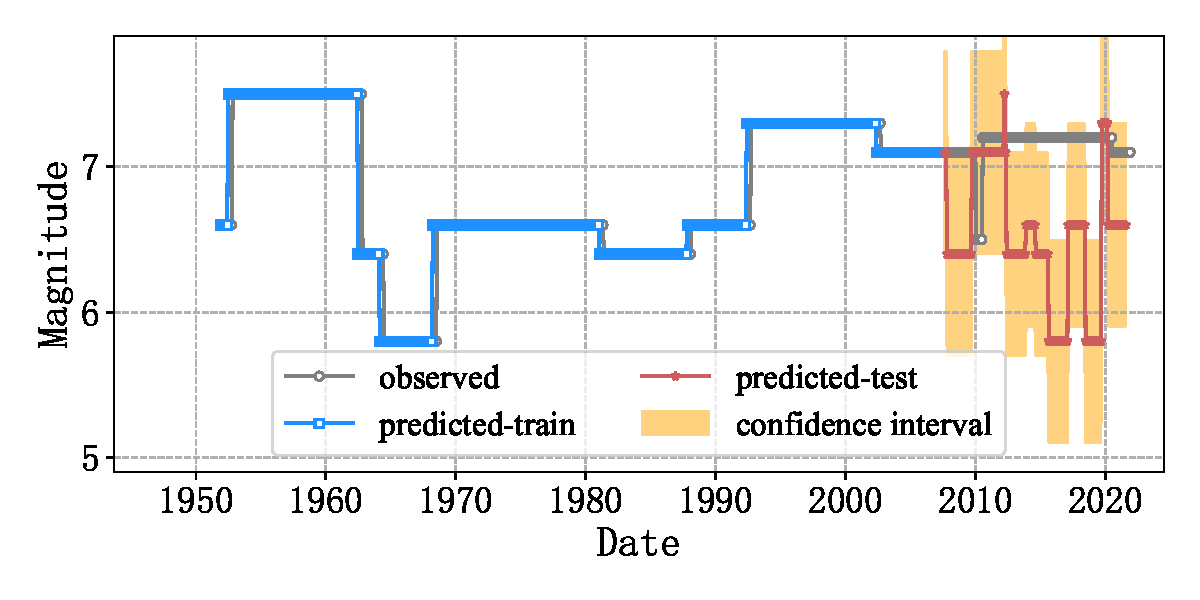
\includegraphics[width=\textwidth]{Img/chap5_seism/future10/seism_etr_minyear_1932_maxyear_2021_spanlat_2_spanlon_4_timewindow_120_nextmonth_120_minmag_3.0_blocks1.pdf}
    \vspace{-1cm}
    \label{fig:seism_etr_minyear_1932_maxyear_2021_spanlat_2_spanlon_4_timewindow_120_nextmonth_120_minmag_3.0_blocks1}
  \end{subfigure}
  \bicaption[不同模型基于整个区块预测未来10年最大震级的时间序列图(数据集划分比例为0.8:0.2)]{不同模型基于整个区块预测未来10年最大震级的时间序列图(数据集划分比例为0.8:0.2)。}{The time series of predicting the maximum magnitute with the split ratio 0.8:0.2 in next ten years by different models.}
  \label{fig:seism_minyear_1932_maxyear_2021_spanlat_2_spanlon_4_timewindow_120_nextmonth_120_minmag_3.0_blocks1}
\end{figure}


表\ref{tab:seism_minyear_1932_maxyear_2021_spanlat_2_spanlon_4_timewindow_120_nextmonth_120_minmag_3.0_blocks1}展示了整个区块在不同模型下预报未来10年最大震级的拟合指标效果。图\ref{fig:seism_minyear_1932_maxyear_2021_spanlat_2_spanlon_4_timewindow_120_nextmonth_120_minmag_3.0_blocks1}展示了整个区块拟合未来10年最大震级的时间序列。图\ref{fig:seism_minyear_1932_maxyear_2021_spanlat_2_spanlon_4_timewindow_120_nextmonth_120_minmag_3.0_blocks1}显示出未来10年最大震级时间序列较为规律,横轴时间$t$代表着未来$[t-10,t]$年时间段内的最大震级。
由表\ref{tab:seism_minyear_1932_maxyear_2021_spanlat_2_spanlon_4_timewindow_120_nextmonth_120_minmag_3.0_blocks1}和图\ref{fig:seism_minyear_1932_maxyear_2021_spanlat_2_spanlon_4_timewindow_120_nextmonth_120_minmag_3.0_blocks1}可知,几种模型仍均出现了很大程度的过拟合现象。同第\ref{sec:seism_result_1}节和第\ref{sec:seism_result_6}节的结论,机器学习对预测加州地区未来10年的最大震级是失败的。

\subsubsection{验证集:测试集=0.85:0.15}\label{sec:seism_result_10_85}

\begin{table}[!htbp]
  \bicaption[不同模型基于整个区块预测未来10年最大震级的拟合指标效果(数据集划分比例为0.85:0.15)]{不同模型基于整个区块预测未来10年最大震级的拟合指标效果(数据集划分比例为0.85:0.15)。}{The metrics for predicting the maximum magnitute with the split ratio 0.85:0.15 in next 10 year by different models.}
  \label{tab:seism_minyear_1932_maxyear_2021_spanlat_2_spanlon_4_timewindow_120_nextmonth_120_minmag_3.0_split_ratio_0.85_blocks1}
  \centering
  \footnotesize
  \begin{tabular}{lcccc}
    \toprule
    \multirow{2}*{模型} & \multicolumn{2}{c}{训练集} & \multicolumn{2}{c}{验证集} \\
    \cmidrule(lr){2-3} \cmidrule(lr){4-5} \noalign{\smallskip}
    & MSE & RMSE & MSE & RMSE \\
    \midrule
    LSTM & 0.0136 & 0.1168 & 0.0469 & 0.2167 \\
    SVR & 0.0212 & 0.1455 & 0.0052 & 0.0723 \\
    LR & 0.0121 & 0.1100 & 0.0250 & 0.1581 \\
    RF & 0.0008 & 0.0287 & 0.1339 & 0.3660 \\
    GBRT & 0.0001 & 0.0110 & 0.1269 & 0.3562 \\
    DT & \textbf{0.0000} & \textbf{0.0000} & 0.0287 & 0.1693 \\
    KNN & \textbf{0.0000} & \textbf{0.0000} & 0.0265 & 0.1627 \\
    ETR & \textbf{0.0000} & \textbf{0.0000} & 0.1021 & 0.3196 \\
    \bottomrule
  \end{tabular}
\end{table}

\begin{figure}[!htbp]
  \vspace{-2cm}
  \centering
  \begin{subfigure}[b]{0.45\textwidth}
    \caption{LSTM}
    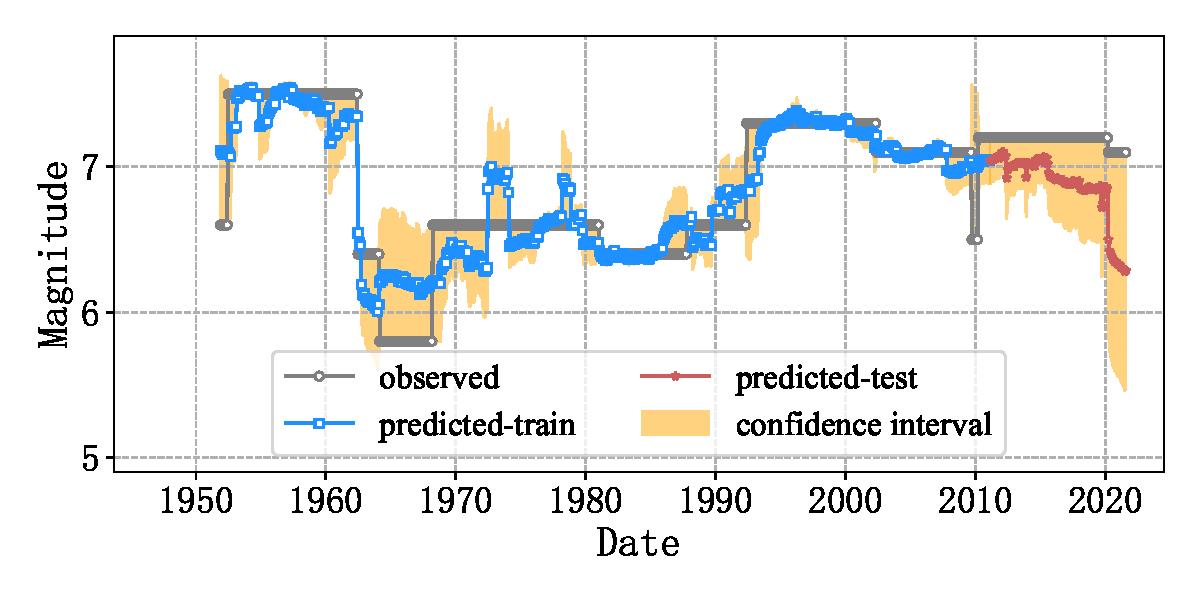
\includegraphics[width=\textwidth]{Img/chap5_seism/split85/seism_lstm_minyear_1932_maxyear_2021_spanlat_2_spanlon_4_timewindow_120_nextmonth_120_minmag_3.0_split_ratio_0.85_blocks1.pdf}
    \vspace{-1cm}
    \label{fig:seism_lstm_minyear_1932_maxyear_2021_spanlat_2_spanlon_4_timewindow_120_nextmonth_120_minmag_3.0_split_ratio_0.85_blocks1}
  \end{subfigure}
  ~
  \begin{subfigure}[b]{0.45\textwidth}
    \caption{SVR} 
    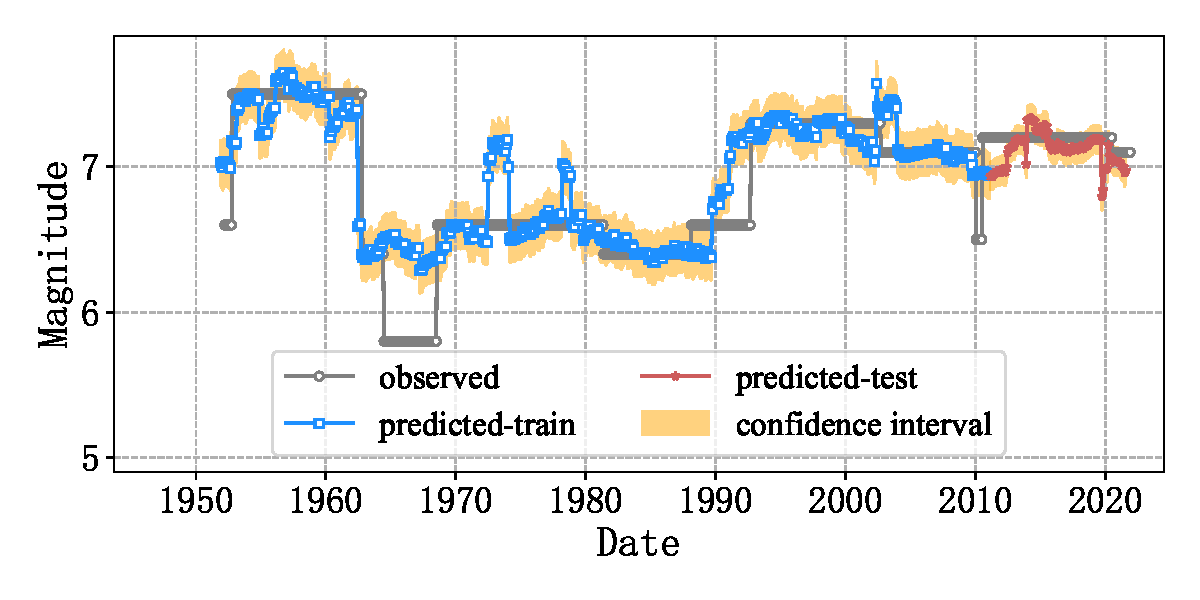
\includegraphics[width=\textwidth]{Img/chap5_seism/split85/seism_svr_minyear_1932_maxyear_2021_spanlat_2_spanlon_4_timewindow_120_nextmonth_120_minmag_3.0_split_ratio_0.85_blocks1.pdf}
    \vspace{-1cm}
    \label{fig:seism_svr_minyear_1932_maxyear_2021_spanlat_2_spanlon_4_timewindow_120_nextmonth_120_minmag_3.0_split_ratio_0.85_blocks1}
  \end{subfigure}   
  \\
  \begin{subfigure}[b]{0.45\textwidth}
      \caption{LR}
      \vspace{-0.2cm}
      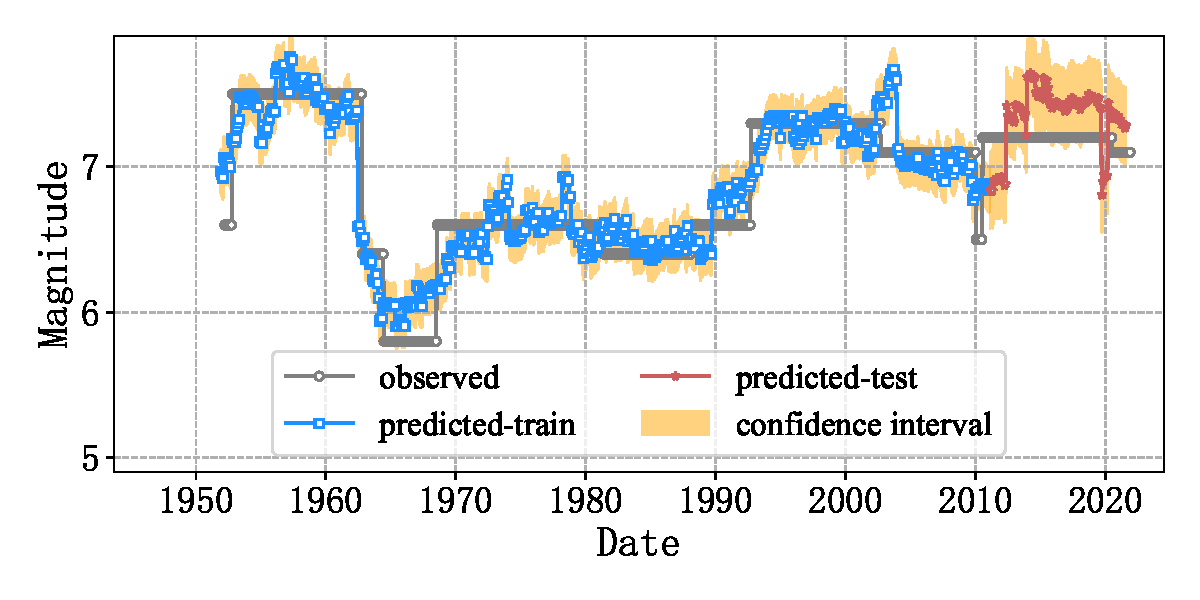
\includegraphics[width=\textwidth]{Img/chap5_seism/split85/seism_lr_minyear_1932_maxyear_2021_spanlat_2_spanlon_4_timewindow_120_nextmonth_120_minmag_3.0_split_ratio_0.85_blocks1.pdf}
      \vspace{-1cm}
      \label{fig:seism_lr_minyear_1932_maxyear_2021_spanlat_2_spanlon_4_timewindow_120_nextmonth_120_minmag_3.0_split_ratio_0.85_blocks1}
  \end{subfigure}
  ~
  \begin{subfigure}[b]{0.45\textwidth}
    \caption{RF}
    \vspace{-0.2cm}
    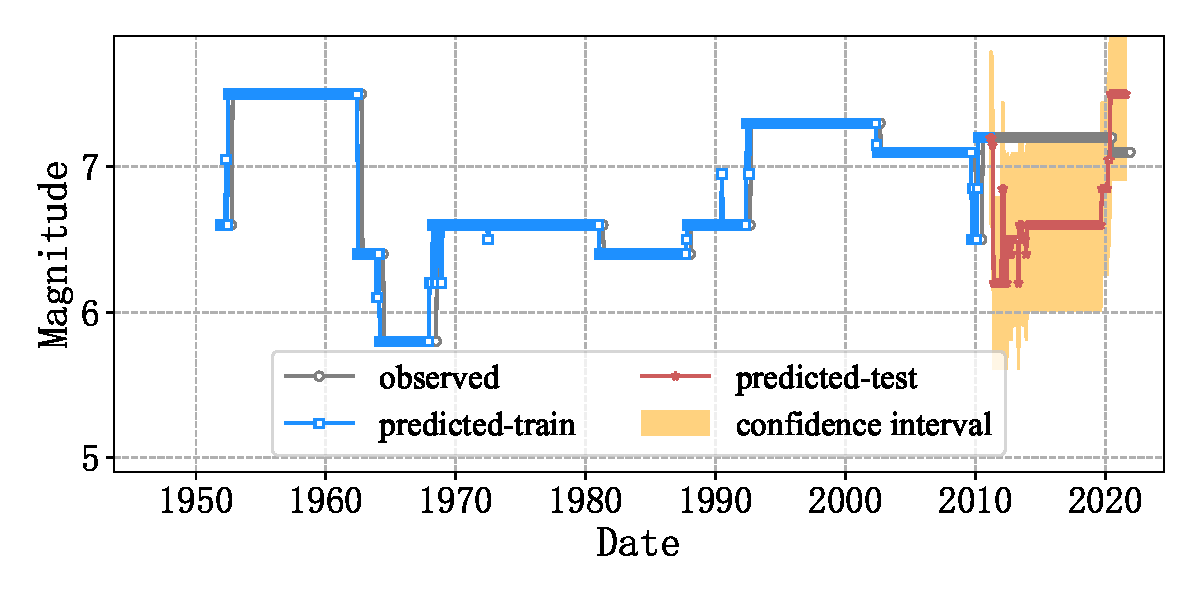
\includegraphics[width=\textwidth]{Img/chap5_seism/split85/seism_rf_minyear_1932_maxyear_2021_spanlat_2_spanlon_4_timewindow_120_nextmonth_120_minmag_3.0_split_ratio_0.85_blocks1.pdf}
    \vspace{-1cm}
    \label{fig:seism_rf_minyear_1932_maxyear_2021_spanlat_2_spanlon_4_timewindow_120_nextmonth_120_minmag_3.0_split_ratio_0.85_blocks1}
  \end{subfigure}
  \\
  \begin{subfigure}[b]{0.45\textwidth}
    \caption{GBRT}
    \vspace{-0.2cm}
    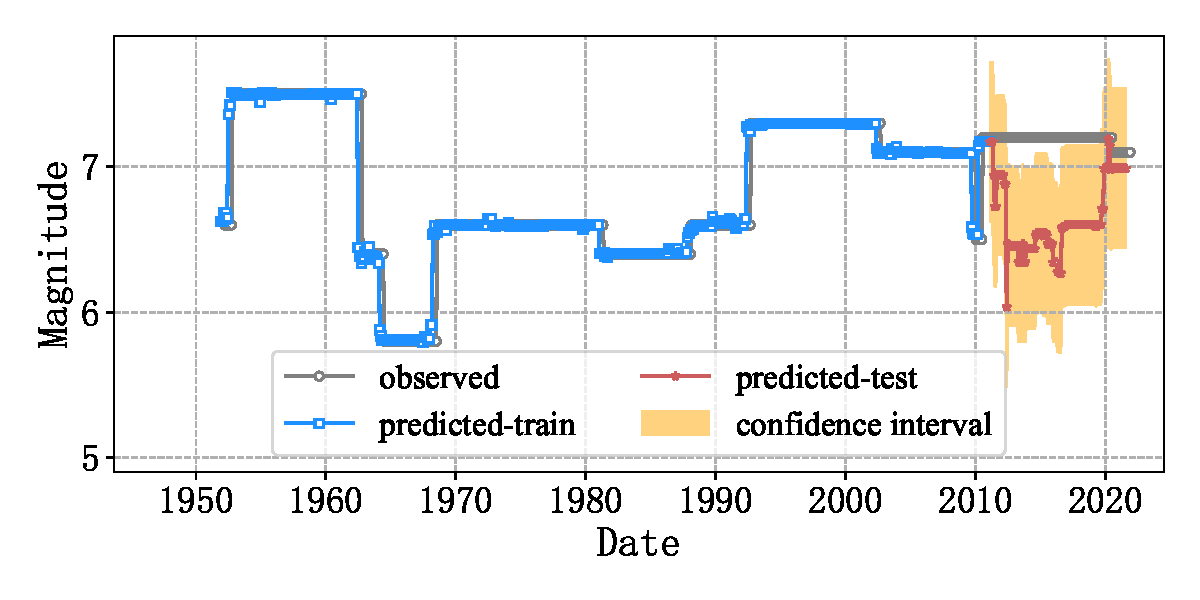
\includegraphics[width=\textwidth]{Img/chap5_seism/split85/seism_gbr_minyear_1932_maxyear_2021_spanlat_2_spanlon_4_timewindow_120_nextmonth_120_minmag_3.0_split_ratio_0.85_blocks1.pdf}
    \vspace{-1cm}
    \label{fig:seism_gbr_minyear_1932_maxyear_2021_spanlat_2_spanlon_4_timewindow_120_nextmonth_120_minmag_3.0_split_ratio_0.85_blocks1}
  \end{subfigure}
  ~
  \begin{subfigure}[b]{0.45\textwidth}
    \caption{DT}
    \vspace{-0.2cm}
    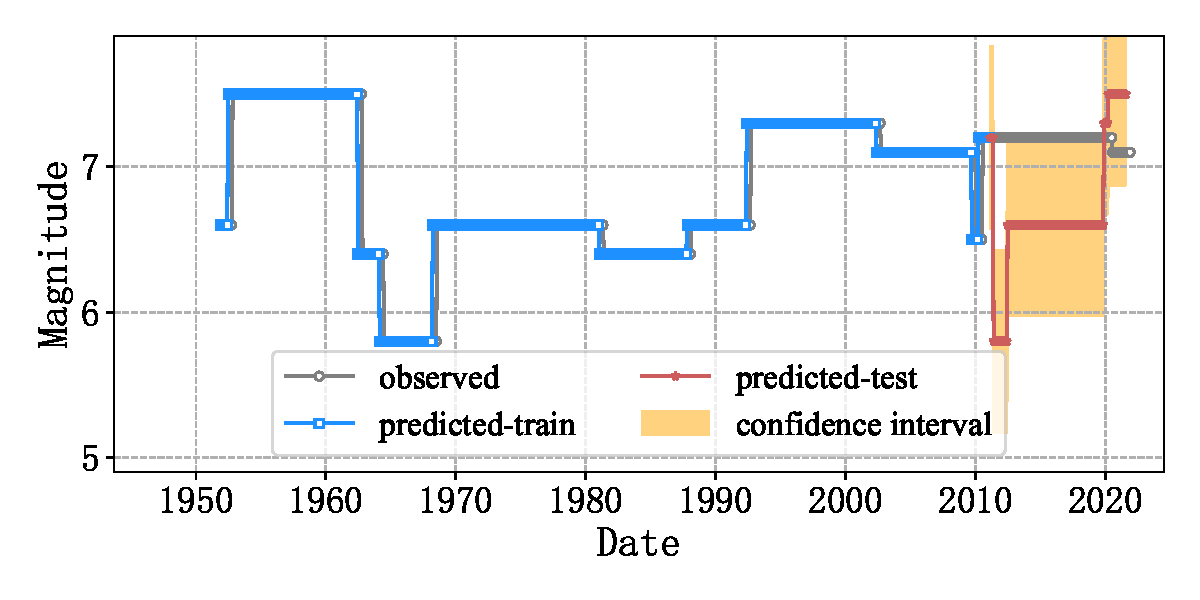
\includegraphics[width=\textwidth]{Img/chap5_seism/split85/seism_dt_minyear_1932_maxyear_2021_spanlat_2_spanlon_4_timewindow_120_nextmonth_120_minmag_3.0_split_ratio_0.85_blocks1.pdf}
    \vspace{-1cm}
    \label{fig:seism_dt_minyear_1932_maxyear_2021_spanlat_2_spanlon_4_timewindow_120_nextmonth_120_minmag_3.0_split_ratio_0.85_blocks1}
  \end{subfigure}
  \\
  \begin{subfigure}[b]{0.45\textwidth}
    \caption{KNN}
    \vspace{-0.2cm}
    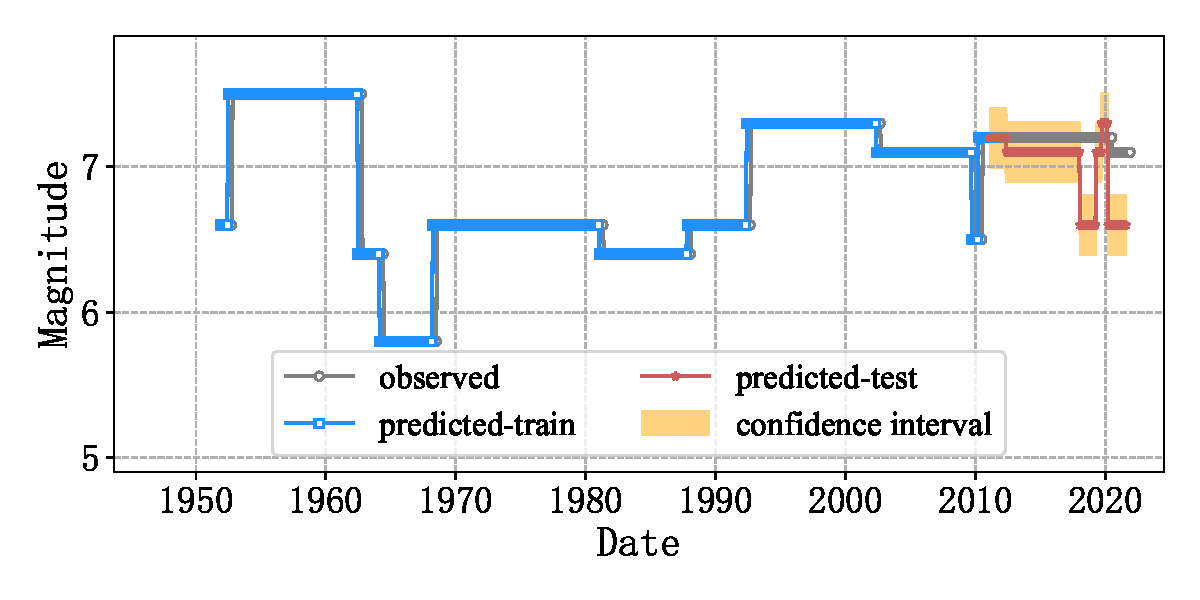
\includegraphics[width=\textwidth]{Img/chap5_seism/split85/seism_kn_minyear_1932_maxyear_2021_spanlat_2_spanlon_4_timewindow_120_nextmonth_120_minmag_3.0_split_ratio_0.85_blocks1.pdf}
    \vspace{-1cm}
    \label{fig:seism_knn_minyear_1932_maxyear_2021_spanlat_2_spanlon_4_timewindow_120_nextmonth_120_minmag_3.0_split_ratio_0.85_blocks1}
  \end{subfigure}
  ~
  \begin{subfigure}[b]{0.45\textwidth}
    \caption{ETR}
    \vspace{-0.2cm}
    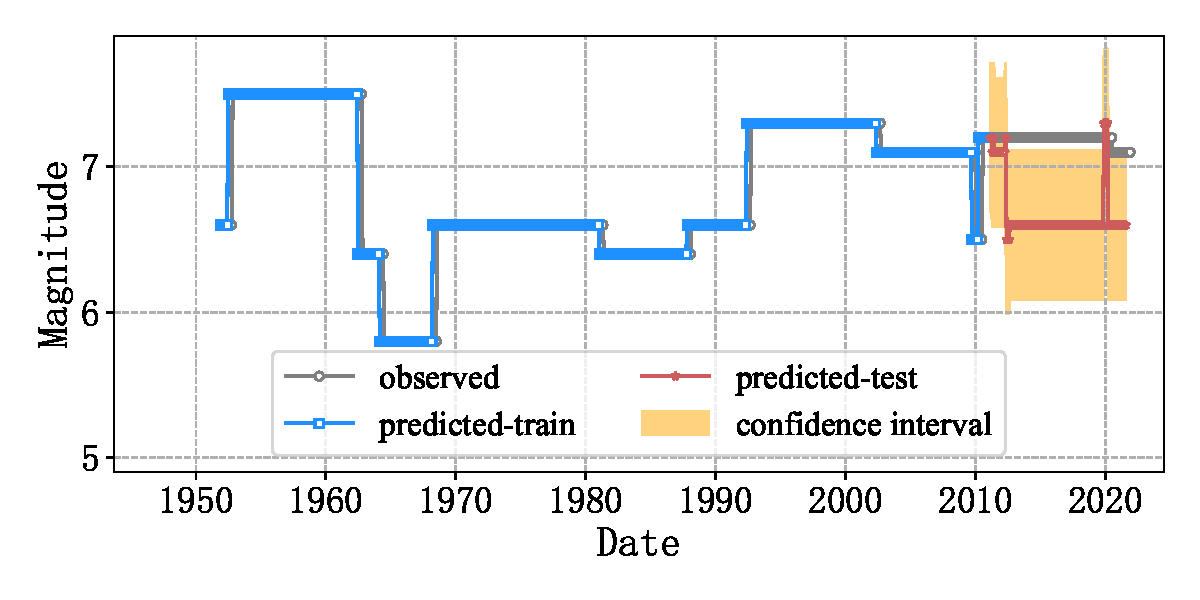
\includegraphics[width=\textwidth]{Img/chap5_seism/split85/seism_etr_minyear_1932_maxyear_2021_spanlat_2_spanlon_4_timewindow_120_nextmonth_120_minmag_3.0_split_ratio_0.85_blocks1.pdf}
    \vspace{-1cm}
    \label{fig:seism_etr_minyear_1932_maxyear_2021_spanlat_2_spanlon_4_timewindow_120_nextmonth_120_minmag_3.0_split_ratio_0.85_blocks1}
  \end{subfigure}
  \bicaption[不同模型基于整个区块预测未来10年最大震级的时间序列图(数据集划分比例为0.85:0.15)]{不同模型基于整个区块预测未来10年最大震级的时间序列图(数据集划分比例为0.85:0.15)。}{The time series of predicting the maximum magnitute with the split ratio 0.85:0.15 in next ten years by different models.}
  \label{fig:seism_minyear_1932_maxyear_2021_spanlat_2_spanlon_4_timewindow_120_nextmonth_120_minmag_3.0_split_ratio_0.85_blocks1}
\end{figure}

这里数据集划分比例为0.85:0.15。表\ref{tab:seism_minyear_1932_maxyear_2021_spanlat_2_spanlon_4_timewindow_120_nextmonth_120_minmag_3.0_split_ratio_0.85_blocks1}展示了整个区块在不同模型下预报未来10年最大震级的拟合指标效果。图\ref{fig:seism_minyear_1932_maxyear_2021_spanlat_2_spanlon_4_timewindow_120_nextmonth_120_minmag_3.0_split_ratio_0.85_blocks1}展示了整个区块拟合未来10年最大震级的时间序列。由表\ref{tab:seism_minyear_1932_maxyear_2021_spanlat_2_spanlon_4_timewindow_120_nextmonth_120_minmag_3.0_split_ratio_0.85_blocks1}和图\ref{fig:seism_minyear_1932_maxyear_2021_spanlat_2_spanlon_4_timewindow_120_nextmonth_120_minmag_3.0_split_ratio_0.85_blocks1}可知,几种机器学习模型仍均出现了很大程度的过拟合现象。相对而言,KNN和SVR能够较好地拟合测试集数据。

\subsubsection{验证集:测试集=0.9:0.1}\label{sec:seism_result_10_90}

\begin{table}[!htbp]
  \bicaption[不同模型基于整个区块预测未来10年最大震级的拟合指标效果(数据集划分比例为0.9:0.1)]{不同模型基于整个区块预测未来10年最大震级的拟合指标效果(数据集划分比例为0.9:0.1)。}{The metrics for predicting the maximum magnitute with the split ratio 0.9:0.1 in next 10 year by different models.}
  \label{tab:seism_minyear_1932_maxyear_2021_spanlat_2_spanlon_4_timewindow_120_nextmonth_120_minmag_3.0_split_ratio_0.90_blocks1}
  \centering
  \footnotesize
  \begin{tabular}{lcccc}
    \toprule
    \multirow{2}*{模型} & \multicolumn{2}{c}{训练集} & \multicolumn{2}{c}{验证集} \\
    \cmidrule(lr){2-3} \cmidrule(lr){4-5} \noalign{\smallskip}
    & MSE & RMSE & MSE & RMSE \\
    \midrule
    LSTM & 0.0210 & 0.1450 & 0.0053 & 0.0728 \\
    SVR & 0.0212 & 0.1455 & 0.0052 & 0.0723 \\
    LR & 0.0123 & 0.1108 & 0.0074 & 0.0860 \\
    RF & 0.0005 & 0.0225 & 0.0179 & 0.1337 \\
    GBRT & 0.0001 & 0.0116 & 0.0068 & 0.0827 \\
    DT & \textbf{0.0000} & \textbf{0.0000} & 0.0096 & 0.0980 \\
    KNN & \textbf{0.0000} & \textbf{0.0000} & 0.0178 & 0.1332 \\
    ETR & \textbf{0.0000} & \textbf{0.0000} & 0.0169 & 0.1300 \\
    \bottomrule
  \end{tabular}
\end{table}

\begin{figure}[!htbp]
  \vspace{-2cm}
  \centering
  \begin{subfigure}[b]{0.45\textwidth}
    \caption{LSTM}
    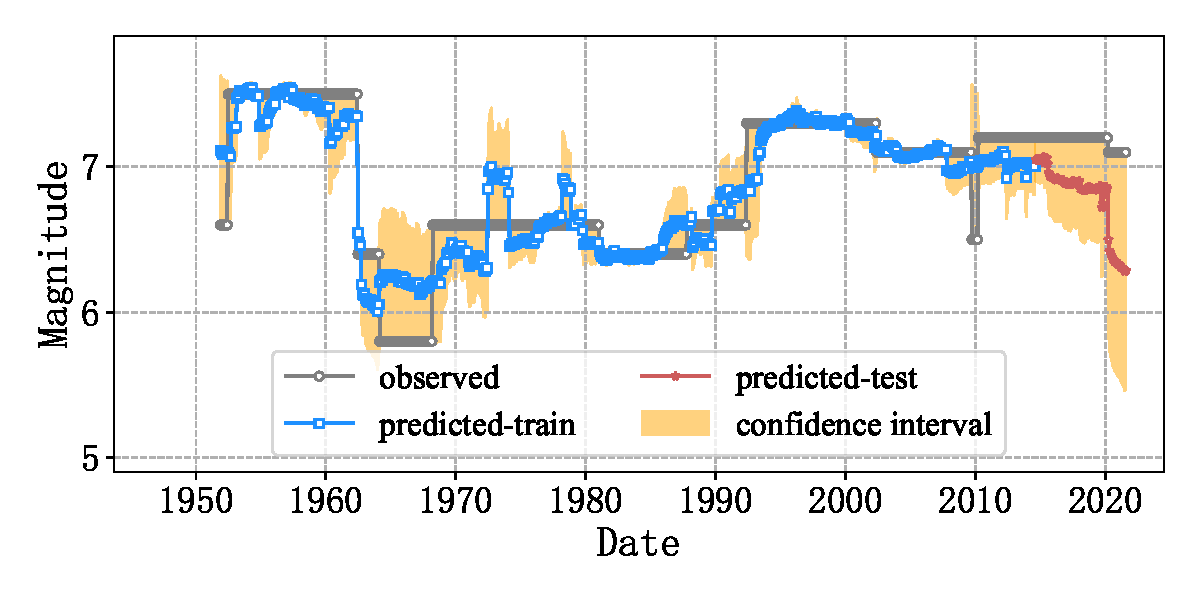
\includegraphics[width=\textwidth]{Img/chap5_seism/split90/seism_lstm_minyear_1932_maxyear_2021_spanlat_2_spanlon_4_timewindow_120_nextmonth_120_minmag_3.0_split_ratio_0.9_blocks1.pdf}
    \vspace{-1cm}
    \label{fig:seism_lstm_minyear_1932_maxyear_2021_spanlat_2_spanlon_4_timewindow_120_nextmonth_120_minmag_3.0_split_ratio_0.9_blocks1}
  \end{subfigure}
  ~
  \begin{subfigure}[b]{0.45\textwidth}
    \caption{SVR} 
    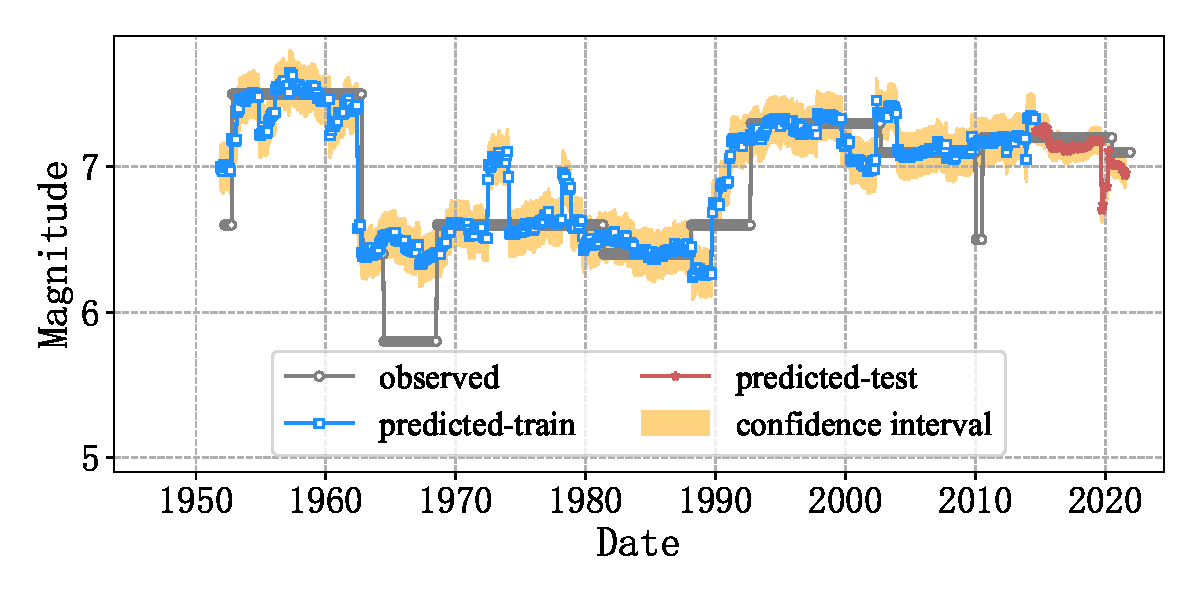
\includegraphics[width=\textwidth]{Img/chap5_seism/split90/seism_svr_minyear_1932_maxyear_2021_spanlat_2_spanlon_4_timewindow_120_nextmonth_120_minmag_3.0_split_ratio_0.9_blocks1.pdf}
    \vspace{-1cm}
    \label{fig:seism_svr_minyear_1932_maxyear_2021_spanlat_2_spanlon_4_timewindow_120_nextmonth_120_minmag_3.0_split_ratio_0.9_blocks1}
  \end{subfigure}   
  \\
  \begin{subfigure}[b]{0.45\textwidth}
      \caption{LR}
      \vspace{-0.2cm}
      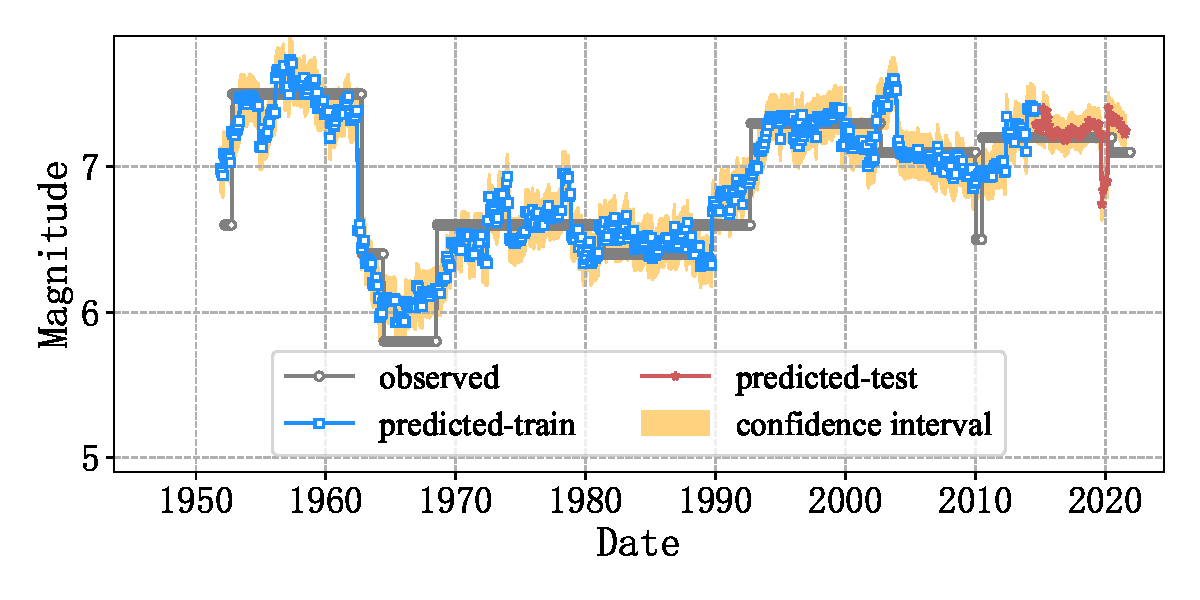
\includegraphics[width=\textwidth]{Img/chap5_seism/split90/seism_lr_minyear_1932_maxyear_2021_spanlat_2_spanlon_4_timewindow_120_nextmonth_120_minmag_3.0_split_ratio_0.9_blocks1.pdf}
      \vspace{-1cm}
      \label{fig:seism_lr_minyear_1932_maxyear_2021_spanlat_2_spanlon_4_timewindow_120_nextmonth_120_minmag_3.0_split_ratio_0.9_blocks1}
  \end{subfigure}
  ~
  \begin{subfigure}[b]{0.45\textwidth}
    \caption{RF}
    \vspace{-0.2cm}
    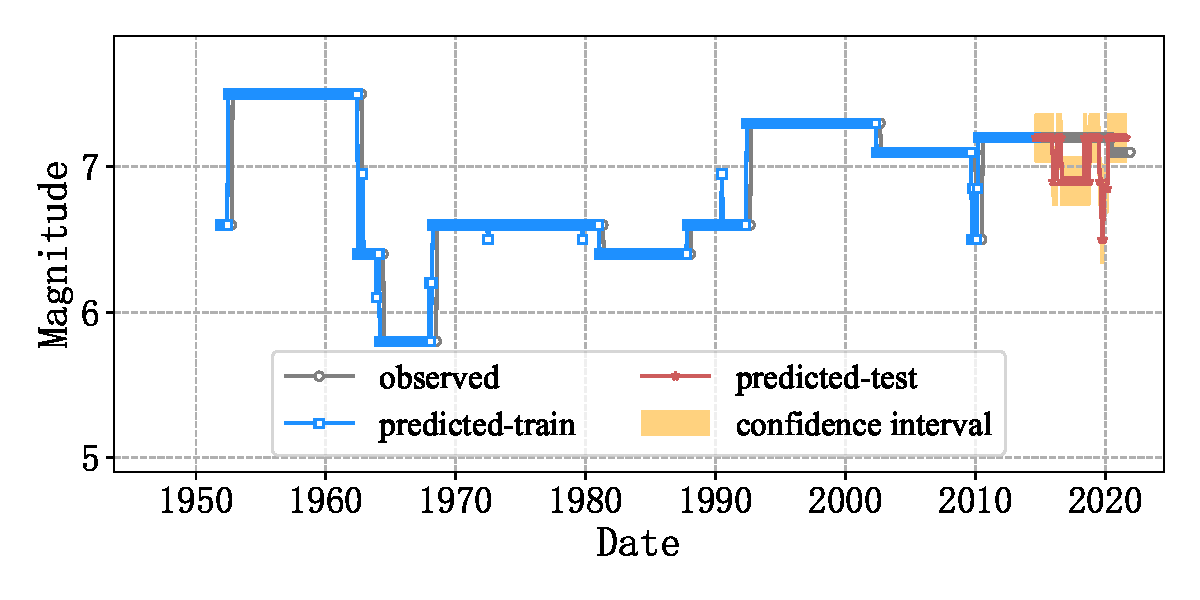
\includegraphics[width=\textwidth]{Img/chap5_seism/split90/seism_rf_minyear_1932_maxyear_2021_spanlat_2_spanlon_4_timewindow_120_nextmonth_120_minmag_3.0_split_ratio_0.9_blocks1.pdf}
    \vspace{-1cm}
    \label{fig:seism_rf_minyear_1932_maxyear_2021_spanlat_2_spanlon_4_timewindow_120_nextmonth_120_minmag_3.0_split_ratio_0.9_blocks1}
  \end{subfigure}
  \\
  \begin{subfigure}[b]{0.45\textwidth}
    \caption{GBRT}
    \vspace{-0.2cm}
    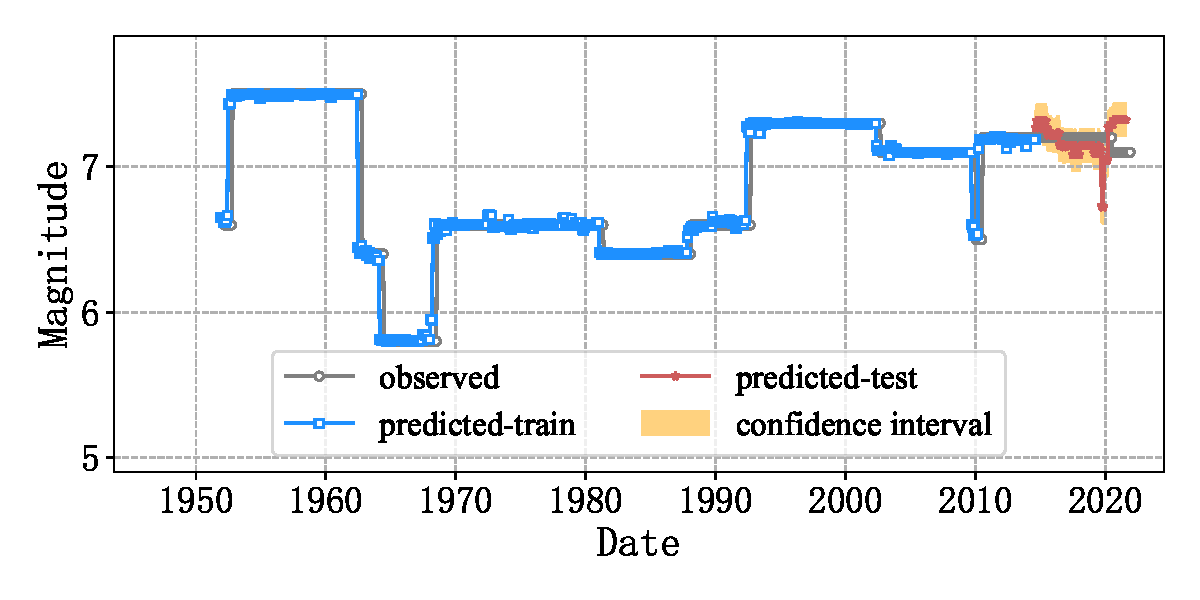
\includegraphics[width=\textwidth]{Img/chap5_seism/split90/seism_gbr_minyear_1932_maxyear_2021_spanlat_2_spanlon_4_timewindow_120_nextmonth_120_minmag_3.0_split_ratio_0.9_blocks1.pdf}
    \vspace{-1cm}
    \label{fig:seism_gbr_minyear_1932_maxyear_2021_spanlat_2_spanlon_4_timewindow_120_nextmonth_120_minmag_3.0_split_ratio_0.9_blocks1}
  \end{subfigure}
  ~
  \begin{subfigure}[b]{0.45\textwidth}
    \caption{DT}
    \vspace{-0.2cm}
    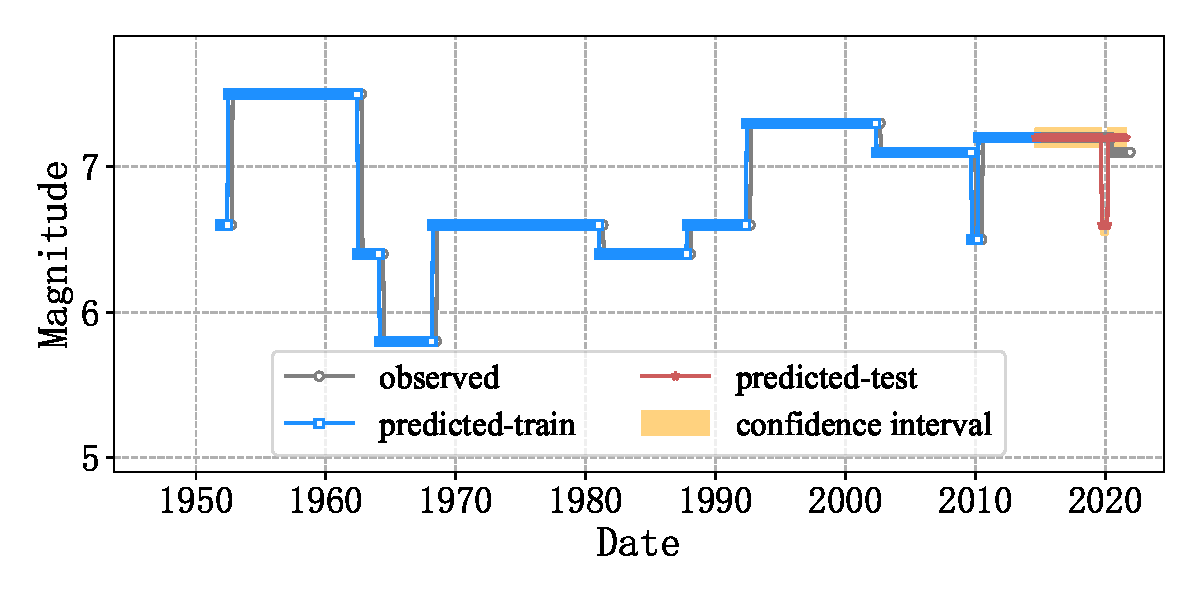
\includegraphics[width=\textwidth]{Img/chap5_seism/split90/seism_dt_minyear_1932_maxyear_2021_spanlat_2_spanlon_4_timewindow_120_nextmonth_120_minmag_3.0_split_ratio_0.9_blocks1.pdf}
    \vspace{-1cm}
    \label{fig:seism_dt_minyear_1932_maxyear_2021_spanlat_2_spanlon_4_timewindow_120_nextmonth_120_minmag_3.0_split_ratio_0.9_blocks1}
  \end{subfigure}
  \\
  \begin{subfigure}[b]{0.45\textwidth}
    \caption{KNN}
    \vspace{-0.2cm}
    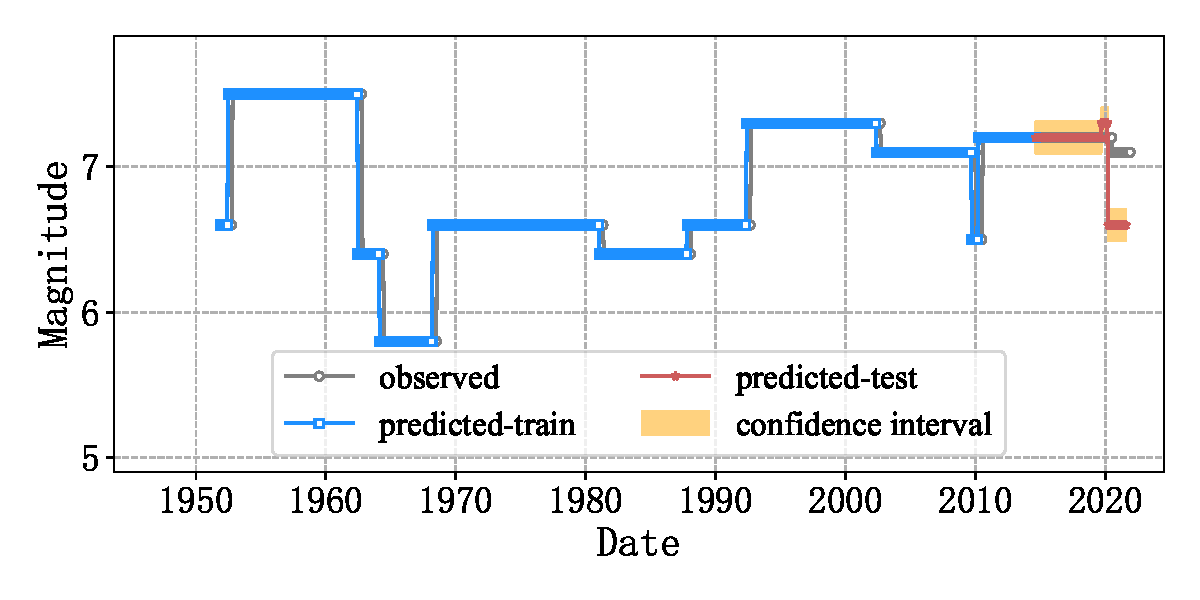
\includegraphics[width=\textwidth]{Img/chap5_seism/split90/seism_kn_minyear_1932_maxyear_2021_spanlat_2_spanlon_4_timewindow_120_nextmonth_120_minmag_3.0_split_ratio_0.9_blocks1.pdf}
    \vspace{-1cm}
    \label{fig:seism_knn_minyear_1932_maxyear_2021_spanlat_2_spanlon_4_timewindow_120_nextmonth_120_minmag_3.0_split_ratio_0.9_blocks1}
  \end{subfigure}
  ~
  \begin{subfigure}[b]{0.45\textwidth}
    \caption{ETR}
    \vspace{-0.2cm}
    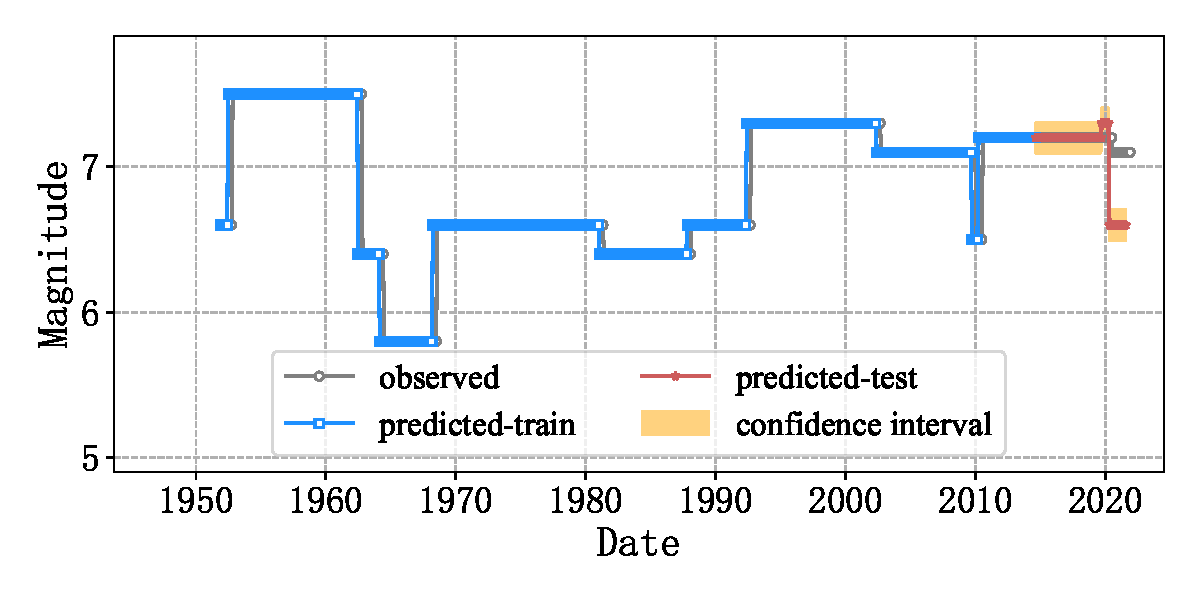
\includegraphics[width=\textwidth]{Img/chap5_seism/split90/seism_etr_minyear_1932_maxyear_2021_spanlat_2_spanlon_4_timewindow_120_nextmonth_120_minmag_3.0_split_ratio_0.9_blocks1.pdf}
    \vspace{-1cm}
    \label{fig:seism_etr_minyear_1932_maxyear_2021_spanlat_2_spanlon_4_timewindow_120_nextmonth_120_minmag_3.0_split_ratio_0.9_blocks1}
  \end{subfigure}
  \bicaption[不同模型基于整个区块预测未来10年最大震级的时间序列图(数据集划分比例为0.9:0.1)]{不同模型基于整个区块预测未来10年最大震级的时间序列图(数据集划分比例为0.9:0.1)。}{The time series of predicting the maximum magnitute with the split ratio 0.9:0.1 in next ten years by different models.}
  \label{fig:seism_minyear_1932_maxyear_2021_spanlat_2_spanlon_4_timewindow_120_nextmonth_120_minmag_3.0_split_ratio_0.90_blocks1}
\end{figure}

这里数据集划分比例为0.9:0.1。表\ref{tab:seism_minyear_1932_maxyear_2021_spanlat_2_spanlon_4_timewindow_120_nextmonth_120_minmag_3.0_split_ratio_0.90_blocks1}展示了整个区块在不同模型下预报未来10年最大震级的拟合指标效果。图\ref{fig:seism_minyear_1932_maxyear_2021_spanlat_2_spanlon_4_timewindow_120_nextmonth_120_minmag_3.0_split_ratio_0.90_blocks1}展示了整个区块拟合未来10年最大震级的时间序列。由表\ref{tab:seism_minyear_1932_maxyear_2021_spanlat_2_spanlon_4_timewindow_120_nextmonth_120_minmag_3.0_split_ratio_0.90_blocks1}可知,出现过拟合的模型有RF、GBRT、DT、KNN、ETR,出现欠拟合的模型有LSTM-RNN、SVR、LR。从图\ref{fig:seism_minyear_1932_maxyear_2021_spanlat_2_spanlon_4_timewindow_120_nextmonth_120_minmag_3.0_split_ratio_0.90_blocks1}可以看出,处了LSTM-RNN,其他几种机器学习模型均能拟合出测试集中7.1级的地震。尽管如此,这几种机器学习方法稳健性很差,数据的略微变动就会影响模型性能。

\subsection{基于整个区块预测未来10年的最大震级范围}\label{sec:seism_result_10_class}

以上均是基于回归的基础上构建机器学习模型,且绝大多数模型拟合的结果均出现了过拟合现象。这里我们尝试将预测未来10年的最大震级看作是分类问题,从不同的角度去观测数据集变化对结果的影响程度。\citet{nan2019xinjiang}指出,地震震级通常可允许的误差为\pm 0.3。本节对震级大小进行等级分类,具体分类情况如表\ref{tab:seism_class}所示,将[3.0,3.2]分为第1类,[3.3,3.5]为第2类,\ldots,大于等于7.5为第16类,共将标签分成16个不同等级类别。  

\begin{table}[!htbp]
  \centering
  \bicaption[震级分类及标签]{震级分类及标签。}{Magnitude classification and labels.}
  \label{tab:seism_class}
  \footnotesize
  \begin{tabular}{cccccccc}
    \toprule
    标签 & 震级 & 标签 & 震级 & 标签 & 震级 & 标签 & 震级 \\
    \midrule
    1 & [3.0,3.2] & 2 & [3.3,3.5] & 3 & [3.6,3.8] & 4 & [3.9,4.1] \\
    5 & [4.2,4.4] & 6 & [4.5,4.7] & 7 & [4.8,5.0] & 8 & [5.1,5.3] \\
    9 & [5.4,5.6] & 10 & [5.7,5.9] & 11 & [6.0,6.2] & 12 & [6.3,6.5] \\
    13 & [6.6,6.8] & 14 & [6.9,7.1] & 15 & [7.2,7.4] & 16 & \ge 7.5 \\
    \bottomrule
  \end{tabular}
\end{table}

这里同样采取8种不同类型的模型,分别为LSTM-RNN、支持向量分类器(Support Vector Classification,简称SVC)、线性分类器(Linear Classification,简称LC)、RF、梯度提升分类树(Gradient Boosting Classification Tree,简称GBCT)、DT、KNN、极端树分类器(Extra Trees Classification,简称ETC)。模型输入是6个区块在某个特定时刻前6年时间窗口内的16个地震因子,即输入为$6\times 16=96$个,输出是某个区块下一年的最大震级范围。数据集划分比例为0.8:0.2。针对两层的LSTM-RNN,第一层含64个LSTM神经元,最后一层为全连接层。因这里是分类问题,损失函数采取交叉熵误差函数(见式\ref{eq:ml_cee}),预测精度采取准确度(见式\ref{eq:ml_acc})。同时对16种不同的标签采取one-hot编码。one-hot编码是将分类变量表示为二进制变量。这就要求将分类值映射到整数值,然后每个整数值都表示为一个二进制向量,除了用1标记的整数值的索引外,其余值都是0。

\begin{table}[!htbp]
  \bicaption[不同模型基于整个区块预测未来10年最大震级范围的拟合指标效果(数据集划分比例为0.8:0.2)]{不同模型基于整个区块预测未来10年最大震级范围的拟合指标效果(数据集划分比例为0.8:0.2)。}{The metrics for predicting the ranges of maximum magnitute with the split ratio 0.8:0.2 in next ten years by different models.}
  \label{tab:seism_minyear_1932_maxyear_2021_spanlat_2_spanlon_4_timewindow_120_nextmonth_120_minmag_3.0_split_ratio_0.8_blocks1_class}
  \centering
  \footnotesize
  \begin{tabular}{lcccc}
    \toprule
    \multirow{2}*{模型} & \multicolumn{2}{c}{训练集} & \multicolumn{2}{c}{验证集} \\
    \cmidrule(lr){2-3} \cmidrule(lr){4-5} \noalign{\smallskip}
    & 交叉熵误差 & 精确度 & 交叉熵误差 & 精确度 \\
    \midrule
    LSTM & 0.2891 & 0.7593 & 3.1773 & 0.1488 \\
    SVC & & 0.9432 & & 0.1488 \\
    LC & & 0.9238 & & 0.1488 \\
    RF & & 0.9895 & & 0.1310 \\
    GBCT & & 1.0000 & & 0.4048 \\
    DT & & 1.0000 & & 0.4107 \\
    KNN & & 1.0000 & & 0.1845 \\
    ETC & & 1.0000 & & 0.2857 \\
    \bottomrule
  \end{tabular}
\end{table}

\begin{figure}[!htbp]
  \vspace{-2cm}
  \centering
  \begin{subfigure}[b]{0.45\textwidth}
    \caption{LSTM}
    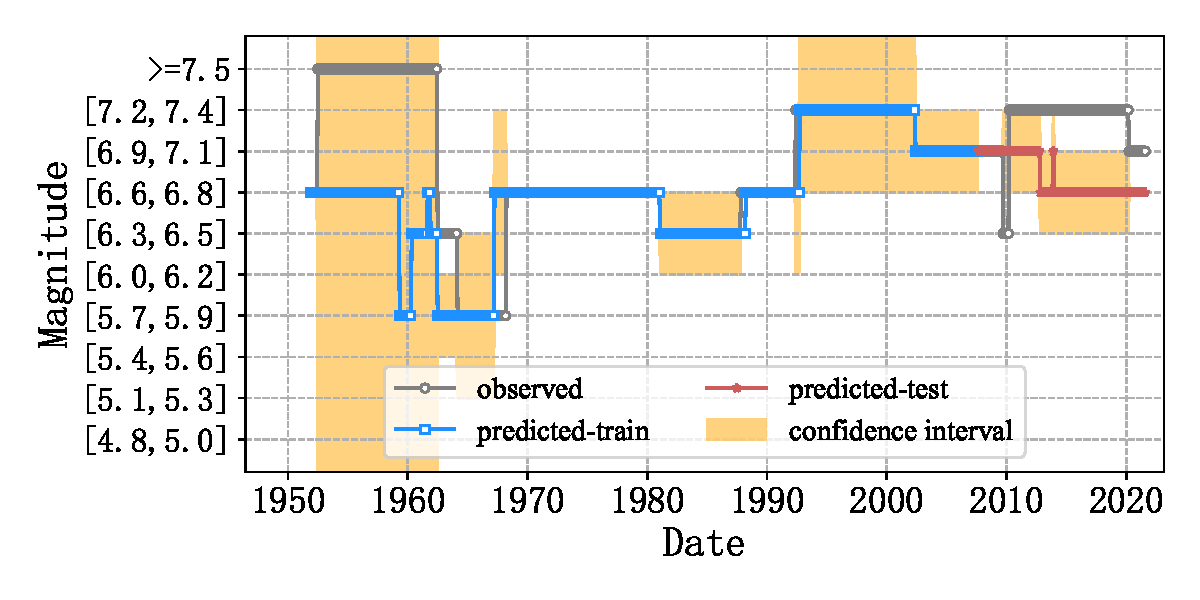
\includegraphics[width=\textwidth]{Img/chap5_seism/future10_class/seism_lstm_minyear_1932_maxyear_2021_spanlat_2_spanlon_4_timewindow_120_nextmonth_120_minmag_3.0_split_ratio_0.8_blocks1_class.pdf}
    \vspace{-1cm}
    \label{fig:seism_lstm_minyear_1932_maxyear_2021_spanlat_2_spanlon_4_timewindow_120_nextmonth_120_minmag_3.0_split_ratio_0.8_blocks1_class}
  \end{subfigure}
  ~
  \begin{subfigure}[b]{0.45\textwidth}
    \caption{SVR} 
    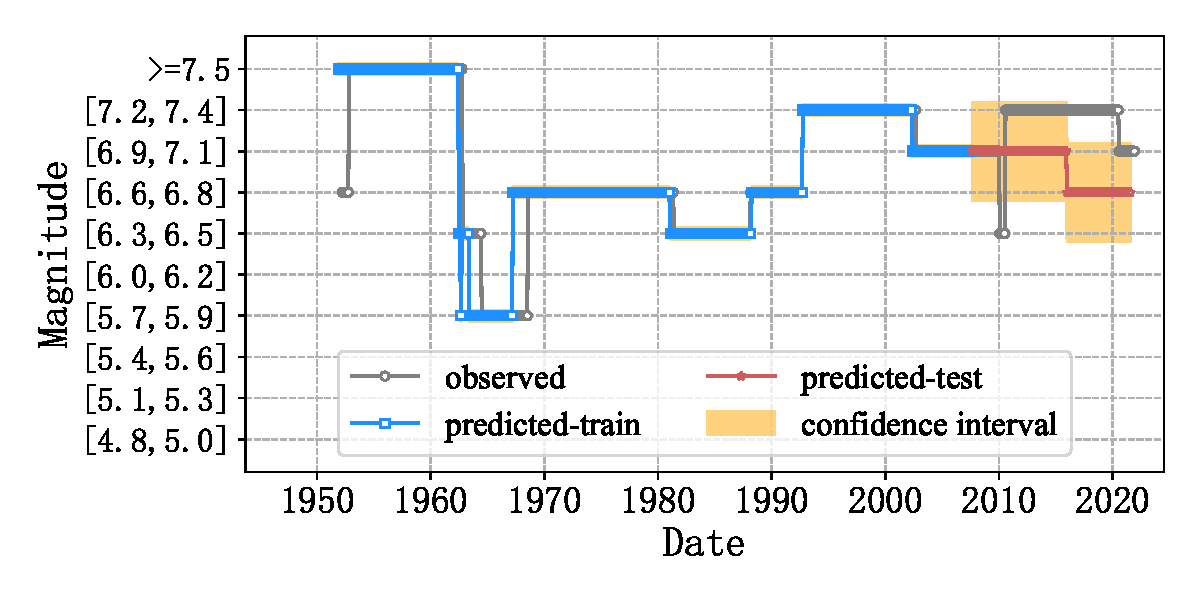
\includegraphics[width=\textwidth]{Img/chap5_seism/future10_class/seism_svr_minyear_1932_maxyear_2021_spanlat_2_spanlon_4_timewindow_120_nextmonth_120_minmag_3.0_split_ratio_0.8_blocks1_class.pdf}
    \vspace{-1cm}
    \label{fig:seism_svr_minyear_1932_maxyear_2021_spanlat_2_spanlon_4_timewindow_120_nextmonth_120_minmag_3.0_split_ratio_0.8_blocks1_class}
  \end{subfigure}   
  \\
  \begin{subfigure}[b]{0.45\textwidth}
      \caption{LR}
      \vspace{-0.2cm}
      \includegraphics[width=\textwidth]{Img/chap5_seism/future10_class/seism_lr_minyear_1932_maxyear_2021_spanlat_2_spanlon_4_timewindow_120_nextmonth_120_minmag_3.0_split_ratio_0.8_blocks1_class.pdf}
      \vspace{-1cm}
      \label{fig:seism_lr_minyear_1932_maxyear_2021_spanlat_2_spanlon_4_timewindow_120_nextmonth_120_minmag_3.0_split_ratio_0.8_blocks1_class}
  \end{subfigure}
  ~
  \begin{subfigure}[b]{0.45\textwidth}
    \caption{RF}
    \vspace{-0.2cm}
    \includegraphics[width=\textwidth]{Img/chap5_seism/future10_class/seism_rf_minyear_1932_maxyear_2021_spanlat_2_spanlon_4_timewindow_120_nextmonth_120_minmag_3.0_split_ratio_0.8_blocks1_class.pdf}
    \vspace{-1cm}
    \label{fig:seism_rf_minyear_1932_maxyear_2021_spanlat_2_spanlon_4_timewindow_120_nextmonth_120_minmag_3.0_split_ratio_0.8_blocks1_class}
  \end{subfigure}
  \\
  \begin{subfigure}[b]{0.45\textwidth}
    \caption{GBRT}
    \vspace{-0.2cm}
    \includegraphics[width=\textwidth]{Img/chap5_seism/future10_class/seism_gbr_minyear_1932_maxyear_2021_spanlat_2_spanlon_4_timewindow_120_nextmonth_120_minmag_3.0_split_ratio_0.8_blocks1_class.pdf}
    \vspace{-1cm}
    \label{fig:seism_gbr_minyear_1932_maxyear_2021_spanlat_2_spanlon_4_timewindow_120_nextmonth_120_minmag_3.0_split_ratio_0.8_blocks1_class}
  \end{subfigure}
  ~
  \begin{subfigure}[b]{0.45\textwidth}
    \caption{DT}
    \vspace{-0.2cm}
    \includegraphics[width=\textwidth]{Img/chap5_seism/future10_class/seism_dt_minyear_1932_maxyear_2021_spanlat_2_spanlon_4_timewindow_120_nextmonth_120_minmag_3.0_split_ratio_0.8_blocks1_class.pdf}
    \vspace{-1cm}
    \label{fig:seism_dt_minyear_1932_maxyear_2021_spanlat_2_spanlon_4_timewindow_120_nextmonth_120_minmag_3.0_split_ratio_0.8_blocks1_class}
  \end{subfigure}
  \\
  \begin{subfigure}[b]{0.45\textwidth}
    \caption{KNN}
    \vspace{-0.2cm}
    \includegraphics[width=\textwidth]{Img/chap5_seism/future10_class/seism_kn_minyear_1932_maxyear_2021_spanlat_2_spanlon_4_timewindow_120_nextmonth_120_minmag_3.0_split_ratio_0.8_blocks1_class.pdf}
    \vspace{-1cm}
    \label{fig:seism_knn_minyear_1932_maxyear_2021_spanlat_2_spanlon_4_timewindow_120_nextmonth_120_minmag_3.0_split_ratio_0.8_blocks1_class}
  \end{subfigure}
  ~
  \begin{subfigure}[b]{0.45\textwidth}
    \caption{ETR}
    \vspace{-0.2cm}
    \includegraphics[width=\textwidth]{Img/chap5_seism/future10_class/seism_etr_minyear_1932_maxyear_2021_spanlat_2_spanlon_4_timewindow_120_nextmonth_120_minmag_3.0_split_ratio_0.8_blocks1_class.pdf}
    \vspace{-1cm}
    \label{fig:seism_etr_minyear_1932_maxyear_2021_spanlat_2_spanlon_4_timewindow_120_nextmonth_120_minmag_3.0_split_ratio_0.8_blocks1_class}
  \end{subfigure}
  \bicaption[不同模型基于整个区块预测未来10年最大震级范围的时间序列图(数据集划分比例为0.8:0.2)]{不同模型基于整个区块预测未来10年最大震级范围的时间序列图(数据集划分比例为0.8:0.2)。}{The time series of predicting the ranges of maximum magnitute with the split ratio 0.8:0.2 in next ten years by different models.}
  \label{fig:seism_minyear_1932_maxyear_2021_spanlat_2_spanlon_4_timewindow_120_nextmonth_120_minmag_3.0_split_ratio_0.8_blocks1_class}
\end{figure}

表\ref{tab:seism_minyear_1932_maxyear_2021_spanlat_2_spanlon_4_timewindow_120_nextmonth_120_minmag_3.0_split_ratio_0.8_blocks1_class}展示了整个区块在不同模型下预报未来10年最大震级的拟合指标效果。图\ref{fig:seism_minyear_1932_maxyear_2021_spanlat_2_spanlon_4_timewindow_120_nextmonth_120_minmag_3.0_split_ratio_0.8_blocks1_class}展示了整个区块拟合未来10年最大震级的时间序列。图\ref{fig:seism_minyear_1932_maxyear_2021_spanlat_2_spanlon_4_timewindow_120_nextmonth_120_minmag_3.0_split_ratio_0.8_blocks1_class}显示出未来10年最大震级时间序列较为规律,横轴时间$t$代表着未来$[t-10,t]$年时间段内的最大震级。
由表\ref{tab:seism_minyear_1932_maxyear_2021_spanlat_2_spanlon_4_timewindow_120_nextmonth_120_minmag_3.0_split_ratio_0.8_blocks1_class}和图\ref{fig:seism_minyear_1932_maxyear_2021_spanlat_2_spanlon_4_timewindow_120_nextmonth_120_minmag_3.0_split_ratio_0.8_blocks1_class}可知,几种模型仍均出现了很大程度的过拟合现象。同第\ref{sec:seism_result_10}节的结论,机器学习对预测加州地区未来10年的最大震级是失败的。

\section{讨论与小结}\label{sec:seism_conclusion}

第\ref{sec:ml_fitting}节详细介绍了过拟合产生的原因。模型的泛化误差来源于偏差、方差和噪声。假设输入地震特征因子向量为$\Vector{X}$,输出未来1年最大震级为$M_{\text{predicted}}$,实际发生震级为$M_{\text{observed}}$,要拟合的目标函数为$f(\Vector{X})$,训练函数为$\hat{f}(\Vector{X})$,则偏差为:
\begin{equation}\adddotsbeforeeqnnum
  \label{eq:seism_bias}
  \text{Bais}^2(\Vector{X})=(\hat{f}(\Vector{X})-M_{\text{observed}})^2.
\end{equation}
高偏差意味着训练集中预测的未来最大震级$M_{\text{predicted}}$与实际发生的最大震级$M_{\text{observed}}$差距大,因此会导致欠拟合的问题。根据第\ref{sec:seism_result}节的结果,训练集中的$M_{\text{predicted}}$与$M_{\text{observed}}$差距较小,不存在欠拟合问题。偏差越小,模型越能充分拟合训练数据集。

与偏差不同,方差度量了训练集的变动导致学习性能的变化,即刻画了数据扰动所造成的影响。它是由训练样本的小波动敏感而导致的误差。方差可以理解为模型预报震级的变化范围,可表达为:
\begin{equation}\adddotsbeforeeqnnum
  \label{eq:seism_variance}
  \text{Variance}(\Vector{X})=E[(\hat{f}(\Vector{X})-f(\Vector{X}))^2].
\end{equation}
高方差意味着训练的模型$\hat{f}(\Vector{X})$与期望模型$f(\Vector{X})$差距大,因此会导致过拟合问题。根据第\ref{sec:seism_result}的结果,测试集中的$M_{\text{predicted}}$与$M_{\text{observed}}$差距较大,方差很大,即模型存在过拟合问题。方差越大,数据扰动产生的影响越大。可能的原因有:模型过于复杂,以至于拟合了训练集中的噪声;训练样本过少;输入特征缺乏代表性等。

除了偏差与方差,噪声也会影响到模型性能的好坏。噪声表达了在预测震级时算法所能达到的期望泛化误差的下界,刻画了学习问题本身的难度。期望预报$f(\Vector{X})$与真实值$M_{\text{observed}}$之间的误差称为噪声,即
\begin{equation}\adddotsbeforeeqnnum
  \label{eq:seism_noise}
  \text{Noise}(\Vector{X})=E[(f(\Vector{X})-M_{\text{observed}})^2].
\end{equation}
当存在噪声时,复杂的模型会尽量覆盖噪声点。即使训练误差很小,由于没有描绘真实的数据趋势,测试误差反而会更大。如果数据是由未知的某个非常复杂的模型产生的,实际上有限的数据集也很难去“代表”这个复杂模型。采用不恰当的数据集拟合,模型性能很难得到提升,因为部分数据在不恰当的复杂假设就像是“噪声”。一般来讲,噪声难以避免,更难以被剔除。训练样本噪声的干扰,导致模型拟合了这些噪声。

从第\ref{sec:seism_result}节来看,无论是哪种机器学习模型,即便采取正则化、Dropout、早停等防止过拟合的策略,过拟合的现象并未好转。因此,模型复杂度不是过拟合产生的根本原因。经过观察发现,部分模型在小震时预报偏大,大震时预报偏小。小震预报偏大可能是因为小震缺失,大震预报偏小可能是统计的时段不够长或需要更多的大震数据。数据长度问题暂时难以解决,只能通过时间的积累才能获取更长时间的地震记录。

地震目录基本不存在噪声。几十年前的地震仪对小震反应可能不灵敏,小震容易被忽视。在地震目录还是由人工记录时,可能会存在误记或漏记。当然,小震不是关注的重点。还有一方面的噪声来自人工地震的影响。但是噪声对本章研究的影响实际上微乎其微。还需要重点考虑训练样本过少、输入特征缺乏代表性等方面。


































% \subsection{评价指标}\label{sec_seism:评价指标}

% 为了评价模型,使用了混淆矩阵(见\ref{tab:seism_confusion_matrix})。其中的四个指标可以描述为:
% \begin{enumerate}
% \item[1] 真阳性( True positives,简称TP)。在未来的一段时间内,模型触发警报且确实发生了地震的地震事件数量;
% \item[2] 真阳性( True negatives,简称TN)。在未来的一段时间内,模型没有触发警报且没有发生地震的地震事件数量;
% \item[3] 真阳性(False positives,简称FP)。在未来的一段时间内,模型触发警报但没有发生地震的地震事件数量;
% \item[4] 真阳性(False negatives,简称FN)。在未来的一段时间内,模型没有触发警报但发生了地震的地震事件数量。
% \end{enumerate}
  
% \begin{table}[!ht]
% \bicaption[混淆矩阵]{混淆矩阵。}{Confusion matrix.}
% \label{tab:seism_confusion_matrix}
% \centering
% \footnotesize
%   \begin{tabular}{cccc}
%   \toprule
%   & &  \multicolumn{2}{c}{观测} \\  
%   \cmidrule(r){3-4} 
%  \noalign{\smallskip} 
%   & & True & False \\
%   \midrule
%   \multirow{2}{*}{预报} & Positive & TP & FP \\
%     & Negative & FN & TN  \\
%   \bottomrule
%   \end{tabular} 
% \end{table}

% 在混淆矩阵(表\ref{tab:seism_confusion_matrix})中,TP和TN值越大,且FP和FN值越小,则模型的性能越好。然而,混淆矩阵里面统计的是个数,面对大量的数据,凭借计算个数,很难衡量模型的优劣。因此在混淆矩阵基本的统计结果上又延伸了几个指标,也称作二级指标\ref{tab:seism_extended_indicators}。

% \begin{table}[!ht]
% \bicaption[几个延伸的衡量指标]{几个延伸的衡量指标。}{Several extended prediction model evaluation indicators.}
% \label{tab:seism_extended_indicators}
% \centering
% \footnotesize
% \resizebox{\textwidth}{!}{
%   \begin{tabular}{llll}
%   \toprule
%   序号 & 指标 & 公式 & 描述 \\
%   \midrule
%   1 & 准确率 & Accuracy=$\displaystyle \frac{\text{TP+TN}}{\text{TP+TN+FP+FN}}$ &
%   所有判断正确的结果占总观测值的百分比。
%   \\ 
%   2 & & $P_0=\displaystyle \frac{\text{TN}}{\text{TN+FN}}$ & 阴性预报值。
%   \\ 
%   3 & 精确率 & Precision=$P_1=\displaystyle \frac{\text{TP}}{\text{TP+FP}}$ &  阳性预报值。
%   \\ 
%   4 & 召回率 & Recall=$S_n=\displaystyle \frac{\text{TP}}{\text{TP+FN}}$ & 敏感性或正确识别的实际阳性率。
%   \\  
%   5 & 特异度 & Specificity=$S_p=\displaystyle \frac{\text{TN}}{\text{TN+FP}}$ &  特异性或正确识别的实际阴性率。
%   \\ 
%   6 & 综合平均值 & Avg=$\displaystyle {\frac{1}{4}}(P_0+P_1+S_n+S_p)$ & 前四个指标的算术平均值。
%   \\ 
%   7 & MCC & $\text{MCC}={\frac{\text{TP\; TN-FP\; FN}}{\sqrt{\text{(TP+TN)(TP+FN)(TN+FP)(TN+FN)}}}}$ &  MCC(Matthew's Correlation Coefficient)为平衡了混淆矩阵四个基本指标。
%   \\ 
%   8 & $F_1$ & $F_1=\displaystyle {\frac{2}{\displaystyle \frac{1}{P_1}+\frac{1}{S_n}}}$ & 精确率和召回率的调和平均数。
%   \\ 
%   9 & $R$& \multicolumn{2}{l}{$\displaystyle R=P_0-S_p+1=S_n-P_1+1$}
%   \\
%   \bottomrule
%   \end{tabular} }
% \end{table}